%TC: macro \marginfootnote [other]
%TC: envir SCfigure [] other
%TC: macrocount beginSCfigure [figure]
\documentclass[11pt,twoside]{report}
\usepackage{preamble}
\setcounter{chapter}{1}
\graphicspath{{../img/}}
\def\includebibliography{}

\externaldocument{introduction}
\externaldocument{morphometric-framework}
\externaldocument{morphometric-applications}
\externaldocument{resummation}
\externaldocument{aerosols}

\begin{document}
\chapter{Geometry and the liquid state}
\epigraph{It tells me that the Creator used the wrong kind of circles.}{Terry Pratchett, \emph{Pyramids} (1989).}
%\epigraph{It was not certain what significance the ceremony held... but the formality was no less sacred for it being unintelligible.}{Mervyn Peake, \emph{Titus Groan}, (1946).}
\label{chapter:background}

In this chapter we provide a self-contained account of the foundational frameworks underlying the two themes of this thesis: \emph{integral geometry} and \emph{liquid state theory}.
I expect the reader to have a background in statistical physics, so my account of liquid state theory is not intended to be exhaustive; for more in-depth treatments see the references herein.
By contrast, I do \emph{not} expect much familiarity with integral geometry.
Understanding the underlying mathematical detail of this field is not essential to follow the rest of the thesis, so I will focus on the key concepts and notation rather than detailed derivation.

This chapter was assembled from my notes on liquid state theory over the previous few years, which I wanted to organise in one place mostly for my own benefit.
As such, this chapter is a little long so I anticipate the expert reader will skim over it; to facilitate this I have placed the important results in boxes as a guide to the most relevant parts.

As many-body correlation functions are a central theme of the results chapters, I have emphasised correlation functions in section \ref{sec:liquid-structure} on liquid structure to the point where I have somewhat belaboured giving the explicit forms and normalisations of the various correlation functions.
Even though we will only use one particular hierarchy of correlation functions in the results chapters, I personally found it helpful to have these formulas in one place.
I have found myself frequently revisiting the transformations between the various hierarchies of correlation functions, so I include them in anticipation that someone repeating or extending this work may profit from having a kind of ``cheat sheet''.

\section[Integral geometry. Or ``How long is a piece of string?'']{Integral geometry\\ {\large Or ``How long is a piece of string?''}}
\label{sec:integral-geometry}

\subsection{Towards a geometric interpretation of extensivity}

Geometry has been a recurring theme in physical theories, appealing because of its intuitive nature.
There are many ways that geometric ideas can be incorporated, but our focus will be on expansions of thermodynamic quantities in terms of \emph{sizes}.
The usefulness of this particular focus is directly connected to the familiar concept of \emph{extensivity} in statistical mechanics, which we will use to guide the following discussion.
Thermodynamic potentials must be extensive to remain well-defined in the thermodynamic limit,
%Defining an extensive quantity as one that scales proportionally to system size, the first meaning of size that comes to mind is probably the volume.
so by focusing on extensive quantities we ensure a thermodynamically consistent description in this limit.

%The first notion of size that likely comes to mind is the volume, though we will generalise to all reasonable notions of size.
%The simplest example we can give is from statistical mechanics: an \emph{extensive variable} is one that scales proportionally to the system volume.
%For a finite system $K \subset \mathbb{R}^d$ %the volume is expressed
%% \begin{equation}
%%   V[K] = \int_K d\vec{r}.
%% \end{equation}
%Then,
As an example, extensive quantities include the \emph{entropy} of a large system which can be expressed in terms of system volume as
\begin{equation*}
  S = s V
\end{equation*}
where $s$ would be an entropy density which is \emph{intensive}, meaning it does not change with system volume.
Another example is the surface energy
\begin{equation*}
  E = \gamma A
\end{equation*}
where $\gamma$ is the surface tension and $A$ is the surface area.
More refined notions define a variable as extensive if it is a \emph{first-order homogeneous function} of any linearly independent set of (different) extensive variables characterising the system size \cite{Chandler1987}.
That is, a variable $\phi$ is extensive if
\begin{equation}\label{eq:extensive-homogeneity}
  \phi(\lambda Y_1, \cdots, \lambda Y_n)
  =
  \lambda \phi(Y_1, \cdots, Y_n)
\end{equation}
where $\{Y_1, \cdots, Y_n\}$ are a complete (linearly independent) set of extensive variables describing the system size.
We will explore what other reasonable notions of `size' there may be, in effect finding a complete set of extensive variables, in the hope that we arrive at ideas which prove useful in developing new theories.

We introduced the area above as a size descriptor for a surface.
Borrowing ideas from differential geometry, we can also characterise the surface's shape through \emph{curvature}.
A surface is a two-dimensional manifold so its local shape is described by two basis vectors.
Supposing the surface is parameterised by coordinates $(x_1, x_2)$, then the basis vectors at a point on the surface $\vec{r}$ are
\begin{equation}
  \vec{e}_\alpha := \frac{\partial \vec{r}}{\partial x_\alpha}
  \qquad \alpha \in \{1, 2\}.
\end{equation}
Then, the shape of the surface is characterised by changes in the basis vectors leading to the curvature tensor
\begin{equation}
  \kappa_{\alpha \beta} := \frac{\partial \vec{e}_\beta}{\partial x_\alpha}
  \qquad \alpha, \beta \in \{1, 2\}.
\end{equation}
The values of the curvature tensor will depend on the choice of coordinate system $(x_1, x_2)$, so it is usual to consider the \emph{curvature invariants}, i.e.\ the trace and determinant%
\marginfootnote{This argument is readily generalised to $(d-1)$-dimensional surfaces in $\mathbb{R}^d$, where we would find $d-1$ invariants of the curvature tensor.},
leading to the the \emph{mean} and \emph{Gaussian curvatures}
\begin{subequations}
  \begin{align}
    H &:= \frac{\Tr{\kappa}}{2}, \\
    G &:= \det{\kappa}.
  \end{align}
\end{subequations}
As an example of how curvature can be a useful concept in statistical mechanics, we put forward the Young-Laplace equation which writes the pressure difference between two fluids as
\begin{equation*}
  \Delta p = 2 \gamma H,
\end{equation*}
with applications to e.g.\ phase coexistence \cite{YoungPTRSL1805,Laplace1805} or frost damage to porous solids \cite{EverettTFS1961}.
Extensive curvature measures are obtained by integrating the curvature invariants over the surface, leading to the integrated mean and Gaussian curvatures $C$ and $X$.

Together, the extensive geometric variables we have introduced so far can be written as%
\marginfootnote{We use the usual physicist abuse of notation where $V$ refers to both a region in space $V \subset \mathbb{R}^3$, and also the physical volume of this space.}
\begin{subequations}\label{eq:intrinsic-volumes-surface-integrals}
  \begin{align}
    \label{eq:volume-measure}
    V
    &=
    \int_V \, d\vec{r},
    \\
    A
    &=
    \int_{\partial V} \, d\vec{r},
    \\
    C
    &=
    \int_{\partial V} H(\vec{r}) \, d\vec{r},
    \\
    X
    &=
    \int_{\partial V} G(\vec{r}) \, d\vec{r}.
  \end{align}
\end{subequations}
The latter three quantities are \emph{expressed} here as the surface integrals, but we shall see that they are really size measures on the volume $V$.
These clearly form a linearly independent set%
\marginfootnote{This can be quickly determined by considering their units, i.e.\ $V: [\si{\metre^3}]$, $A: [\si{\metre^2}]$, $C: [\si{\metre^1}]$, $X: [\si{\metre^0}]$.},
but less obvious is the fact that these are the \emph{only} reasonable notions of size in three-dimensions.
This is a central finding of \emph{integral geometry}, which we will expand on in subsequent sections.
%is a powerful tool for incorporating intuitive, flexible ideas into theories.
%For this reason geometric approaches are common in statistical mechanics such as the Young-Laplace equation, which corrects Asakura-Ozawa
A consequence of this is that together $\{V, A, C, X\}$ form a complete basis for system size in three dimensions, so we could redefine an extensive quantity as one which can be written
\begin{equation}\label{eq:extensive-integral-geometry}
  \phi = a_3 V + a_2 A + a_1 C + a_0 X,
\end{equation}
which, as a linear relation, clearly obeys \eqref{eq:extensive-homogeneity} during the transformation%
\marginfootnote{Note: the rescaling of $\lambda V$ here refers to rescaling the volume measure \eqref{eq:volume-measure}, \emph{not} the object $V \subset \mathbb{R}^3$; in the latter case we would obtain the (non-extensive) transformation $\{V, A, C, X\} \to \{\lambda V, \lambda^{2/3} A, \lambda^{1/3} C, X\}$.}
$\{V, A, C, X\} \to \{\lambda V, \lambda A, \lambda C, \lambda X\}$.

Integral geometry provides elegant and unified description of sizes, and was crucial in the development of modern theories of hard spheres \cite{RosenfeldPRL1989,KonigPRL2004}, including the main ideas underlying chapters \ref{chapter:morphometric-framework}, \ref{chapter:morphometric-applications} and \ref{chapter:resummation}.
This framework thus provides the route to generalising geometrical theories such as the Asakura-Oosawa model for depletion forces \cite{AsakuraJCP1954,AsakuraJPS1958}, and more generally any free volume theory which expresses an energy in terms of a volume in space.
%Integral geometry generalises the underlying geometric principles of these theories into a unified framework for characterising size.
%% We could argue that fundamentally these theories are based on measuring physical sizes.
%% Integral geometry offers a mathematically rigorous formalism for describing sizes, so presents a possible starting point for free volume theories.
%Ideas from this branch of mathematics were crucial to the development of fundamental measure theory (section \ref{sec:fmt}), so it makes sense to place this before the section on liquid state theory.
As integral geometry is generally unfamiliar to people with a background in physics, we will place emphasis on the concepts and intuition rather than rigour and proofs.
We work mainly from standard texts Refs.\ \cite{Santalo2004,SchneiderACIG1984,Schneider2008,Klain1997}.

\subsection{What do we even mean by size?}
\label{sec:what-is-size}

In order to proceed we must define `size', and specify precisely which objects this definition applies to.
We put forward the following qualities of the measures $V, A, C$ and $X$ which make them intuitive notions of size:
\begin{enumerate}
\item They are invariant with respect to translations and rotations, so that an object's size is independent of the observer.
\item They increase additively, i.e.\ they transform under combination of subsystems via the inclusion/exclusion relation e.g.\ for two objects $K_1$ and $K_2$%
  \marginfootnote{We use the square brace notation $V[\cdot]$ to indicate that the size measures are generalised functions, or \emph{functionals}, of their arguments.}
  \begin{equation}\label{eq:additivity}
    V[K_1 \cup K_2] = V[K_1] + V[K_2] - V[K_1 \cap K_2],
  \end{equation}
  and similar expressions for $A$, $C$, and $X$.
  As corollaries, this property contains the idea that the size of nothing is zero, e.g.\ $V[\emptyset] = 0$, and leads to the homogeneity property of extensive variables \eqref{eq:extensive-homogeneity} through \eqref{eq:extensive-integral-geometry}.
\item They are continuous%
  \marginfootnote{Specifically, in integral geometry this continuity property is with respect to the \emph{Hausdorff metric}.
    Details on this can be found in standard texts, e.g.\ Refs.\ \cite{Santalo2004,SchneiderACIG1984,Schneider2008,Klain1997}.}.
  Loosely speaking, this means that the size measures converge as the object is approximated by increasingly finely meshed polyhedra excluding e.g.\ fractal geometries.
  As a simple intuitive example, the measurement of a length will converge continuously to some number as one uses rulers with progressively finer distance markings.
\end{enumerate}
The final property specifically excludes geometries for which we do not expect there to be any reasonable measurement of size.
These properties are the defining characteristics of more general size measures in integral geometry \cite{Santalo2004, Klain1997}.

%% First we define our objects: sets in Euclidean space.

%% We could completely describe the size of simple objects by completely defining their geometry, e.g.\ the dimensions of a box.
%% This is of course sufficient, however it is not very useful.
%% However, this may not be straightforward for more complex objects, and by abstracting the problem somewhat we can obtain useful theorems etc.
%% We now give a brief justification of the above \emph{ansatzes}, in particular why there are only four terms in the expansion.
%% Radius is the only natural parameter for a sphere, however for more general geometries there might be arbitrarily many parameters so one may wonder if they should be included in a general geometric expansion.

Naively, we might attempt to evaluate the size measures on all subsets $V \subset \mathbb{R}^3$, however this turns out to be too broad a definition.
In particular, this leads to the \emph{Banach-Tarski paradox} in which an object can be broken into two, then recomposed through rigid transformations into two objects identical to the original one  \cite{BanachFM1924}; by \eqref{eq:additivity}, a paradox ensues where the original volume is equal to twice itself.
A better definition is the restriction to \emph{polyconvex sets}%
\marginfootnote{The set of polyconvex objects is also sometimes called the \emph{convex ring}.}: objects formed by countable union of \emph{compact} and \emph{convex} objects.
By compact, we mean objects which are
\begin{enumerate}
\item \emph{bounded}, so they must be finite in scope, as no meaningful size can be defined for a body spanning an infinite region of space, and
\item \emph{closed}, so they contain their boundary.
  %, so the surface exists on which measures $\{A,C,X\}$ are defined.
  %This is an important property which we will see by example in discussing the Gauss-Bonnet theorem below.
\end{enumerate}
We write the collection of objects in $d$-dimensions which are compact and convex as $\mathcal{K}^d$.
This class of objects covers most physically relevant geometries, excluding geometries where size measures may be pathological such as those with fractal structures.
%The empty set $\emptyset$ is a compact body, albeit a special case with zero size.
%Compact convex set $K \in \mathcal{K}$ notation.

%% The first intuitive notion for a size: the size of nothing is zero, i.e.:
%% where $\emptyset$ is the empty set.
%% A box: take the largest length, but then the `size' is not increased by modifying its smallest dimensions.
%% Ideally, we want a size measure that increases monotonically as we add additional material. This leads to additivity:
%% \begin{equation}
%%   \phi(A \cup B) = \phi(A) + \phi(B) - \phi(A \cap B)
%% \end{equation}
%% Connection with entropy, leads to homogeneity in arguments which is the building block for extensivity of a thermodynamic potential.
%% This provides a geometrically precise foundation for thermodynamic potentials.

As a way of justifying the above claims, and as a segue into other topics, we introduce a (seemingly) new measure: the \emph{Euler characteristic} $\chi$ which simply counts the number of disjoint objects in a set%
\marginfootnote{As an intuitive illustration of why this is a size measure, I like to imagine that the \emph{size} of a pirate's treasure is the \emph{number} of gold coins in their possession, which is the Euler characteristic of their hoard.}.
More precisely, for a compact and convex object $K \in \mathcal{K}^d$ we define the measure such that
\begin{equation}\label{eq:euler-characteristic-definition}
  \chi[K] :=
  \begin{cases}
    1 & \textrm{if } K \ne \emptyset \\
    0 & \textrm{if } K = \emptyset
  \end{cases}
\end{equation}
then for it to behave additively \eqref{eq:additivity} for a disjoint collection of objects $K_1, \cdots, K_N \in \mathcal{K}^d$ with $K_i \cap K_j = \emptyset$ for $i \ne j$ we find
\begin{equation*}
  \chi[K_1 \cup \cdots \cup K_N] = N,
\end{equation*}
so it is a counting measure.
Some modification of its definition as a counting measure is needed in case of overlaps, however for now we focus on the fact that this measure is rigid-motion invariant, additive and continuous; as such, it would seem to be an independent measure.
However, the \emph{Gauss-Bonnet theorem} from differential geometry equates it with the Gaussian curvature through
\begin{equation}\label{eq:gauss-bonnet}
  X[K] = 2\pi \chi[\partial K],
\end{equation}
so it is really a manifestation of a size measure we have already seen.
It is worth emphasising the Euler characteristic in its own right however, as it is a very important \emph{topological invariant} meaning it does not change with continuous geometric deformations.
We state some important properties of the Euler characteristic below.

Compact objects include their boundary, so using the additivity property we can decompose the Euler characteristic on $K \in \mathcal{K}^d$ into surface and interior terms
\begin{equation*}
  \chi[K] = \chi[ \partial K ] + \chi[ \interior(K) ] = 1.
\end{equation*}
Arguing by induction, we find%
\marginfootnote{Briefly, the only compact object in $d=1$ is a line segment, with $\partial K$ as two disjoint points giving $\chi[\partial K] = 2$.
  Then, in arbitrary dimensions one considers cutting the object in two, leading to an iteration formula which gives the stated result.
  Full details can be found in Ref.\ \cite{Klain1997}.}
\begin{subequations}
  \begin{align}
    \chi[ \partial K ] &= 1 + (-1)^d
    \\
    \chi[ \interior(K) ] &= (-1)^{d+1}
  \end{align}
\end{subequations}
Thus the Gauss-Bonnet theorem \eqref{eq:gauss-bonnet}, valid in $d=3$, gives $X = 4\pi$ for convex objects i.e.\ a constant.
By similar arguments, it can be shown that the Euler characteristic is increased by the number of \emph{cavities} in $K$, and decreased by the number of \emph{holes} in $K$ \cite{Klain1997}.
More generally, the Euler characteristic is modified by $(-1)^{\nu+1}$ times the number of $\nu$-dimensional \emph{voids}.

%% Repeat arguments in figures and you obtain the general rule that dividing an $n$-sphere gives two $n-1$-dimensional convex objects and a $n-1$ sphere dividor.
%% This gives us the rule for the Euler characteristic.
%% Euler characteristic describes the topology.

%% \begin{SCfigure}[H]
%%   \missingfigure[figwidth=0.5\linewidth]{$\partial B$}%
%%   \missingfigure[figwidth=0.5\linewidth]{$\partial B$}
%%   \caption{Effect of holes: divide 2d circle in two (2 rods + 2 points).}
%% \end{SCfigure}

%% \begin{SCfigure}[H]
%%   \missingfigure[figwidth=0.5\linewidth]{$\partial B$}%
%%   \missingfigure[figwidth=0.5\linewidth]{$\partial B$}
%%   \caption{Effect of cavities: divide 3d sphere in two (2 discs + circle).}
%% \end{SCfigure}

Having defined what we mean by `size', we can start to introduce some useful results from integral geometry.
This will start with generalisations of the size measures, and their completeness as a vector space for an extensive property \eqref{eq:extensive-homogeneity}.
Then, we will introduce formulas which are useful in evaluating partition functions for hard particle systems.

\subsection{Intrinsic volumes as generalised size measures}

It will sometimes be helpful to use a dimension independent formalism%
\marginfootnote{Specifically, in chapter \ref{chapter:resummation} we will derive a theory for the liquid state.
  In order to obtain results for all physical dimensions $d \le 3$, we will work in arbitrary $d$ and substitute $d \in \{1, 2, 3\}$ at the end of our derivation.},
so it is convenient to introduce generalisations of the geometric parameters $\{V,A,C,X\}$: the \emph{intrinsic volumes} $\{V_d, V_{d-1}, \cdots, V_0\}$.
%\hl{Connect with the curvature measures of differential geometry.}
To introduce the intuition behind these generalised volumes we start from the observation that the quantities $\{V,A,C,X\}$ can be imagined as the size of projections onto $k$-dimensional subspaces in $\mathbb{R}^3$; for a compact body $K \in \mathcal{K}^3$ we have:
\begin{enumerate}
\item $V[K]$ is trivially the volume of the intersection of $K$ with the 3-dimensional subspace i.e.\ all of Euclidean space.
\item $A[K]$ can be thought of as the typical size of two-dimensional images formed by projections onto planes.
\item $C[K]$ is related to the projections onto one-dimensional subspaces i.e.\ lines.
  This curvature measure is normally thought of as a surface property, but this definition suggests an equivalence (up to a different normalisation) with the \emph{mean width} $L[K]$ of the body.
\item $X[K]$ is obtained from projections onto a single point, corroborating the equivalence with the Euler characteristic $\chi[K]$ articulated by the Gauss-Bonnet theorem \eqref{eq:gauss-bonnet}.
\end{enumerate}

\begin{SCtable}
  \begin{minipage}[b]{\linewidth}
    \centering
    \begin{tabular}{ccccc}
      \toprule
      $k$ & $\omega_k$ & $V_k(\ball_1)$ & $V_k(\ball_2)$ & $V_k(\ball_3)$ \\
      \midrule
      0 & 1 & 1 & 1 & 1 \\
      1 & 2 & 2 & $\pi$ & 4 \\
      2 & $\pi$ && $\pi$ & $2\pi$ \\
      3 & $\frac{4\pi}{3}$ &&& $\frac{4\pi}{3}$ \\
      \bottomrule
    \end{tabular}
  \end{minipage}
  \caption{Intrinsic volumes of the $d$-dimensional unit ball $\ball_d$ in physical dimensions $d \le 3$.}
  \label{table:ball-intrinsic-volumes}
\end{SCtable}

Generalising the above intuition to $d$-dimensions, we see that in general we can imagine $d+1$ projections and so expect $d+1$ corresponding volumes.
We define the $k$th intrinsic volume as the average size of the projections onto $k$-dimensional linear subspaces of $\mathbb{R}^d$, i.e.\ \cite{Klain1997,Santalo2004}
%Denoting the space of all $k$ dimensional linear subspaces in $\mathbb{R}^d$ as $\mathrm{Graff}(d,k)$ (the affine Grassmanian), the intrinsic volume is obtained by
\begin{equation}\label{eq:intrinsic-volumes}
  V_k(K)
  =
  C_{k,d-k}
  \int \chi[K \cap E_{d-k}] \, dE_{d-k}
\end{equation}
where the integral is taken over all affine transformations of the plane $E_{d-k}$ in $\mathbb{R}^d$, and flag coefficient
\begin{equation}\label{eq:flag-coefficients}
  C_{k,d-k}
  :=
  \frac{d!}{k! (d-k)!} \frac{\omega_d}{\omega_k \omega_{d-k}},
\end{equation}
where the volume of the $d$-dimensional ball with unit radius $\ball_d$ is
\begin{equation}
  \omega_d := V_d[\ball_d] = \frac{\pi^{d/2}}{\Gamma(\frac{d}{2} + 1)}.
\end{equation}
The flag coefficients $C_{k,d-k}$ have a similar structure to binomial coefficients, and play a similar \emph{combinatorial} role in the combination of geometric objects (section \ref{sec:kinematic-formula}).
By convention, the normalisation of the measure $dE_{d-k}$ in \eqref{eq:intrinsic-volumes} is chosen to give the intrinsic volumes for the unit ball as
\begin{equation}\label{eq:intrinsic-volume-ball}
  V_k [\ball_d]
  =
  {d \choose k} \frac{\omega_d}{\omega_{d-k}},
\end{equation}
with values in physical dimensions $d \le 3$ given in Table~\ref{table:ball-intrinsic-volumes}.
%The intrinsic volumes thus only depend on the dimensionality of the body, not the embedding space.
A set of common geometrical quantities and their reduction to the intrinsic volumes in $d \le 3$ is given in Table~\ref{table:geometric-quantities}.

%% \vspace{0.5em}
%% \begin{tcolorbox}[title=Aside: nomenclature of spheres vs balls]
%%   The terms `sphere' and `ball' are used interchangeably in physics (and colloquially), however in geometry these refer to different things; `ball' refers to the solid object whereas `sphere' refers to its boundary, i.e.\
%%   \begin{equation*}
%%     S_{d-1} = \partial \ball_d,
%%   \end{equation*}
%%   As a surface manifold, the $(d-1)$-dimensionality of the sphere is reduced by one from its original space.
%%   So strictly speaking, when we speak of hard spheres in physics we really mean hard balls.
%%   %% \marginfootnote{Strictly speaking the interactions between hollow spheres and solid balls would be identical, so it is possible to still speak of hard spheres.
%%   %%   However, typically we always exclude geometries where spheres contain each another so hard balls better capture the interactions of interest.
%%   %%   Moreover, colloidal hard spheres are solid.}
%%   %in the geometric sense.
%% \end{tcolorbox}

\vspace{0.5em}
\begin{tcolorbox}[title=Hadwiger's characterisation theorem]
  A classic theorem of integral geometry due to Hadwiger \cite{Hadwiger1957} states that the intrinsic volumes are the \emph{only} class of functionals with the size properties described in section \ref{sec:what-is-size}: rigid-motion invariance, additivity and continuity.
  \vspace{1em}

  A corollary of this theorem is that the intrinsic volumes must form a linear vector space for any functional which also possesses these properties, thus providing the $d$-dimensional generalisation of an extensive variable \eqref{eq:extensive-integral-geometry} as one which adopts the form
  \begin{equation}\label{eq:extensive-integral-geometry-d}
    \phi = \sum_{k=0}^d a_k V_k.
  \end{equation}
\end{tcolorbox}

Exploiting this theorem, we will use the intrinsic volumes to construct theories of the hard sphere liquid in section \ref{sec:fmt} and subsequent chapters.
In the next section we will state some useful results for doing calculations in statistical mechanics with the intrinsic volumes.

\begin{SCtable}
  \begin{minipage}[b]{\linewidth}
    \centering
    \begin{tabular}{ccc}
      \toprule
      \multicolumn{2}{c}{Geometric quantity} \\
      \cmidrule(r){1-2}
      Name & Symbol & Functional \\
      \midrule
      \multicolumn{3}{c}{$d = 1$} \\
      \midrule
      Euler characteristic & $\chi$ & $V_0$ \\
      Length & $L$ & $V_1$ \\
      \midrule
      \multicolumn{3}{c}{$d = 2$} \\
      \midrule
      Euler characteristic & $\chi$ & $V_0$ \\
      Perimeter & $L$ & $2 V_1$ \\
      Area & $A$ & $V_2$ \\
      \midrule
      \multicolumn{3}{c}{$d = 3$} \\
      \midrule
      Euler characteristic & $\chi$ & $V_0$ \\
      Mean width & $L$ & $\frac{1}{2} V_1$ \\
      Mean radius & $R$ & $\frac{1}{4} V_1$ \\
      Surface area & $A$ & $2 V_2$ \\
      Volume & $V$ & $V_3$ \\
      Integrated Gaussian curvature & $X$ & $4 \pi V_0$ \\
      Integrated mean curvature & $C$ & $\pi V_1$ \\
      \bottomrule
    \end{tabular}
  \end{minipage}
  \caption[Common geometrical quantities]{
    Common geometrical quantities and their representation in terms of the intrinsic volumes $\{V_k\}$.
    The intrinsic volumes are morphological measures describing the size of a body.
    The common geometric interpretations of $V_k$ for $k < d$ typically involves integrations over the boundary $\partial K$ rather than $K$ itself, leading to the curvature measures $\{C,X\}$ in $d=3$ giving an equivalent description as one involving Euler characteristic and the typical width $\{\chi, L\}$.
    However, the intrinsic volumes are more general as they can be evaluated for shapes where curvatures are not locally defined, e.g. at lines and vertices.}
  \label{table:geometric-quantities}
\end{SCtable}

%% \subsection{Generalised functions acting on sets}

%% Scalar multiplication or \emph{dilate}:
%% \begin{equation}
%%   \epsilon A = \{\epsilon a : a \in A\}
%% \end{equation}
%% \emph{Minkowski addition}:
%% \begin{equation}
%%   A + B := \{ a + b : a \in A \textrm{ and } b \in B \}
%% \end{equation}
%% \emph{Minkowski difference}:
%% \begin{equation}
%%   A - B := \{ c : c + B \subseteq A \}
%% \end{equation}
%% Note that these operations are not the inverses of each other as in the the case of arithmetic, i.e.\ in general
%% \begin{equation*}
%%   A - B \ne A + (-B).
%% \end{equation*}
%% Instead, set addition and subtraction operations are related through
%% \begin{equation*}
%%   A - B = (A^C + (-B))^C.
%% \end{equation*}

%% %% \begin{SCfigure}[H]
%% %%   \missingfigure[figwidth=0.333\linewidth]{}%
%% %%   \missingfigure[figwidth=0.333\linewidth]{}%
%% %%   \missingfigure[figwidth=0.333\linewidth]{}
%% %%   \caption{Examples of Minkowski addition with ball:
%% %%     ball $\to$ ball,
%% %%     line $\to$ capsule/spherocylinder (common in nature: bacterium?),
%% %%     circle $\to$ torus.
%% %%   }
%% %% \end{SCfigure}

%% \begin{SCfigure}
%%   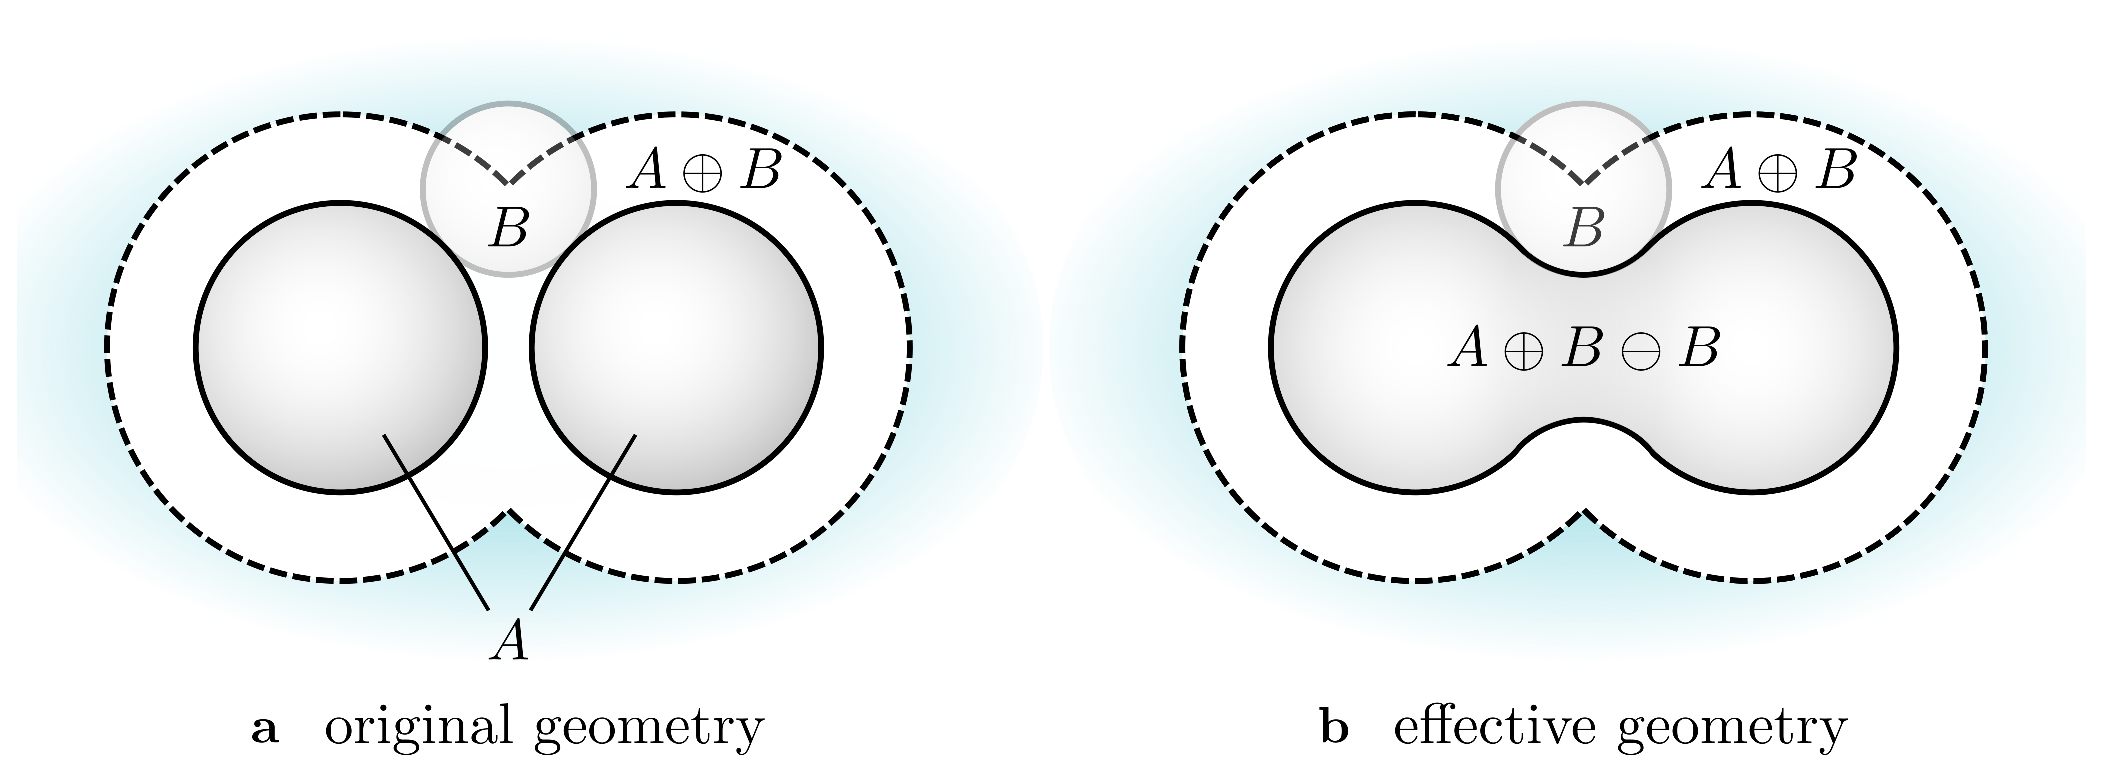
\includegraphics[width=0.9\linewidth,center]{minkowski-addition}
%%   \caption[Minkowski addition and difference]{
%%     Minkowski addition and difference.
%%     Note how these are not inverse operations.}
%% \end{SCfigure}

%% \vspace{0.5em}
%% \begin{tcolorbox}[title=Steiner's formula for parallel volumes]
%%   For a compact, convex body $K \in \mathcal{K}^d$ the parallel volume is expressable as:
%%   \begin{equation}
%%     V_d[K + \epsilon \ball_d] =
%%     \sum_{i=0}^d V_i[K] \omega_{d-i} \epsilon^{d-i}
%%   \end{equation}
%% \end{tcolorbox}

\subsection{Kinematic formulas}
\label{sec:kinematic-formula}

Here we introduce the \emph{kinematic formulas} which calculate hitting probabilities, i.e.\ the probability that randomly distributed objects collide.
This problem is applicable to the evaluation of partition functions in statistical mechanics, of which we will see specific examples in section \ref{sec:fmt} and chapter \ref{chapter:resummation}.

Two compact and convex objects $K_1, K_2 \in \mathcal{K}^d$ overlap if their intersection is non-empty $K_1 \cap K_2 \ne \emptyset$.
The intersection of convex objects is also convex, so from the definition of the Euler characteristic \eqref{eq:euler-characteristic-definition} we can write
\begin{equation*}
  \chi[K_1 \cap K_2]
  =
  \begin{cases}
    1 & \textrm{ if } K_1 \cap K_2 \ne \emptyset \\
    0 & \textrm{ if } K_1 \cap K_2 = \emptyset
  \end{cases}
\end{equation*}
then the probability that the two objects collide is
\begin{equation*}
  \mathrm{Prob} \left[ \textrm{collision} \right]
  =
  \frac{1}{V} \int_V \chi[K_1 \cap K_2(\vec{r})] \, d\vec{r}
\end{equation*}
where $K_2$ is uniformly distributed and $K_1$ acts as a fixed target.
Here, $K_2$ is \emph{translated} over the accessible volume, however in general these objects will be non-spherical so we should also consider the \emph{rotations}.
Integral geometry more naturally deals with integrations over relative positions \emph{and} orientations, at the small cost of additional notation.
%In addition to integrations over particle positions $\{\vec{r}_1, \cdots, \vec{r}_n\}$ we also have to consider their orientations $\{\vec{\theta}_1, \cdots, \vec{\theta}_n\}$ where each $\vec{\theta}_i$ represents an Euler angle tuple.
%Then, assuming an isotropic phase where all orientations are equally likely each positional integral generalises to
Writing the relative orientation as the Euler angle tuple $\vec{\theta}$, we consider the generalisation
\begin{equation*}
  \int_{\mathbb{R}^d} d\vec{r}
  \to
  \int_{\mathbb{R}^d \times SO(d)} d\vec{r} d\vec{\theta}
  :=
  \int_{G_d} dg,
\end{equation*}
with the normalisation in the angular measure such that $\int d\vec{\theta} = 1$.
In the right-most equality we introduced the rigid-motion operation acting on a body $K \in \mathcal{K}^d$ as
\begin{equation*}
  g K := \{\mathcal{R}_\theta \, \vec{k} + \vec{r} \, | \, \vec{k} \in K\},
  %(\mathcal{T} \circ \mathcal{R})(\vec{r}, \vec{\theta}),
\end{equation*}
a member of the rigid motion group $g \in G_d := \mathbb{R}^d \times \mathrm{SO}(d)$, and where $\mathcal{R}_\theta \in \mathrm{SO}(d)$%
\marginfootnote{$\mathrm{SO}(d)$ is the \emph{special orthogonal group}, i.e.\ the group of all orthogonal matrices with unit determinant.}
is the rotation matrix parameterised by $\vec{\theta}$.
Then the generalised measure for particle collisions becomes
\begin{equation*}
  \int_{G_d} \chi[K_1 \cap g K_2] \, dg
\end{equation*}
if they occupy all of Euclidean space.
We will see integrals like this emerge from liquid state theory in sections \ref{sec:virial-series} and \ref{sec:fmt}, and later in chapter \ref{chapter:resummation}.

\vspace{0.5em}
\begin{tcolorbox}[title=Principal kinematic formula]
  %% Noting that $\chi = V_0$ is the lowest order intrinsic volume, the latter line of \eqref{eq:low-density-insertion} is ideally suited to a treatment within integral geometry.
  A central result of integral geometry is the principal kinematic formula of Blaschke and Santal\'o \cite{BlaschkeMZ1936,Blaschke1937,SantaloASI1936} which gives the explicit form of these collisional integrals as \cite{Santalo2004,Klain1997}
  %\cite{Santalo2004,SchneiderACIG1984,Schneider2008,Klain1997}
  \begin{equation}\label{eq:binomial-kinematic-formula}
    \int_{G_d} \chi[K_1 \cap g K_2] \, dg
    =
    \sum_{k=0}^d (C_{k,d-k})^{-1} V_k[K_1] V_{d-k}[K_2]
  \end{equation}
  We see the flag coefficients \eqref{eq:flag-coefficients} play an analogous role here in conjugating the intrinsic volumes as binomial coefficients do in algebraic expansions%
  \marginfootnote{For this reason Klain and Rota argue that integral geometry should be called \emph{continuous combinatorics} \cite{Klain1997}, because it generalises combinatorial results to continuous spaces}.
  More general formulas exist for more general integrals over $V_k[K_1 \cap K_2]$ for all $k$ \cite{Klain1997}, however these do not have an interpretation in terms of evaluating partition functions so we will not be using them.
\end{tcolorbox}

The principal kinematic formula \eqref{eq:binomial-kinematic-formula} can be iterated for the intersections of many bodies $\{K_1, \cdots, K_n\}$ giving \cite{Santalo2004,MarechalPRE2014}
\begin{subequations}\label{eq:multinomial-kinematic-formula}
  \begin{equation}
    \begin{split}
      & \quad
      \int_{G_d^n} \chi[K_1 \cap g_2 K_2 \cap \cdots \cap g_n K_n]
      \, dg_2 \cdots dg_n
      \\ = &
      \sum_{\substack{i_1, \cdots, i_n = 0 \\ i_1 + \cdots + i_n = nd}}^d
      (C_{i_1, \cdots, i_n})^{-1}
      V_{i_1}(K_1)
      \prod_{j=2}^n
      V_{i_j}(K_j)
    \end{split}
  \end{equation}
  \begin{equation}
    \textrm{with} \qquad
    C_{i_1, \cdots, i_n}
    := \frac{1}{i_1! \omega_{i_1}}
    \prod_{j=2}^n
    \left(
    \frac{d!}{i_j!} \frac{\omega_d}{\omega_{i_j}}
    \right)
  \end{equation}
\end{subequations}
where $C_{i_1, \cdots, i_n}$ would be the multinomial generalisation of the flag coefficients \eqref{eq:flag-coefficients}.
We will use this iterated formula in chapter \ref{chapter:resummation} to resum a piece of the virial series (to be introduced in the upcoming section \ref{sec:virial-series}).

%% We have the invariant measure on 1-dimensional linear subspaces of $\mathbb{R}^d$ (\emph{Grassmanians}) as
%% \begin{equation}
%%   [d] = \tau_d(\textrm{Gr}(d,1))
%%   = \frac{d \omega_d}{2 \omega_{d-1}}.
%% \end{equation}
%% Factorial defined as
%% \begin{equation}
%%   [k]! = \prod_{i=0}^k \, [i]
%% \end{equation}
%% Flag coefficients from binomial coefficients
%% \begin{equation}
%%   {d \brack k}
%%   := \frac{[n]!}{[k]! [n-k]!}
%%   = {d \choose k}
%%   \frac{\omega_d}{\omega_k \omega_{d-k}}
%% \end{equation}
%% Provides the generalisation of combinatorial results to continuous spaces.
%% Analagously to binomial coefficients, the flag coefficients obey
%% \begin{equation}\label{eq:flag-coefficients-symmetry}
%%   {d \brack k} = {d \brack d - k}.
%% \end{equation}
%% Note that we can rewrite \eqref{eq:intrinsic-volume-ball} using the flag coefficients as
%% \begin{equation}\label{eq:intrinsic-volume-ball-flag}
%%   \mu_k (\ball_d) = {d \choose k} \frac{\omega_d}{\omega_{d-k}}
%%   = {d \brack k} \omega_k
%% \end{equation}

%% \begin{center}
%% \begin{tabular}{cccccc}
%%   \toprule
%%   $k$ & $\omega_k$ & $[k]$ & $[k]!$ & ${2 \brack k}$ & ${3 \brack k}$ \\
%%   \midrule
%%   0 & 1 & 1 & 1 & 1 & 1 \\
%%   1 & 2 & 1 & 1 & $\frac{\pi}{2}$ & 2 \\
%%   2 & $\pi$ & $\frac{\pi}{2}$ & $\frac{\pi}{2}$ & 1 & 2 \\
%%   3 & $\frac{4\pi}{3}$ & 2 & $\pi$ & & 1 \\
%%   \bottomrule
%% \end{tabular}
%% \end{center}

%% \vspace{0.5em}
%% \begin{tcolorbox}[title=General kinematic formula]
%%   For $0 \le k \le d$:
%%   \begin{equation}
%%     \int_{\mathbb{E}_d} \mu_k (A \cap g B) \, dg =
%%     \sum_{i=0}^{d-k}
%%     {i + k \brack k} {d \brack i}^{-1}
%%     \mu_{i+k}(A) \mu_{d-i}(B)
%%   \end{equation}
%%   \begin{equation*}
%%     \int_{\mathbb{E}_d} \mu_k (A \cap g B) \, dg =
%%     \sum_{i=0}^{d-k}
%%     {i + k \brack k}
%%     {d \brack i + k}
%%     \kappa_{i+k}(A) \kappa_{d-i}(B)
%%   \end{equation*}
%%   In regular binomial:
%%   \begin{equation*}
%%     \int_{\mathbb{E}_d} \mu_k (A \cap g B) \, dg =
%%     \sum_{i=0}^{d-k}
%%     {i + k \choose k} {d \choose i}^{-1}
%%     \frac{\omega_{i+k} \omega_{d-i}}{\omega_k \omega_d}
%%     \mu_{i+k}(A) \mu_{d-i}(B)
%%   \end{equation*}
%% \end{tcolorbox}

%% \begin{equation*}
%%   {n \choose k} {k \choose p}
%%   =
%%   \frac{n!}{k!(n-k)!}
%%   \frac{k!}{p!(k-p)!}
%%   =
%%   \frac{n!}{p!(k-p)!(n-k)!}
%%   =
%%   {n \choose p, k-p, n-k}
%% \end{equation*}
%% I.e. this is a trinomial coefficient.
%% So we have
%% \begin{equation*}
%%   {n \brack k} {k \brack p}
%%   =
%%   {n \choose k}
%%   {k \choose p}
%%   \frac{\omega_n}{\omega_k \omega_{n-k}}
%%   \frac{\omega_k}{\omega_p \omega_{k-p}}
%%   =
%%   {n \choose p, k-p, n-k}
%%   \frac{\omega_n}{\omega_p \omega_{k-p} \omega_{n-k}}
%% \end{equation*}

\section{Statistical physics of fluids}
\label{sec:liquid-state-theory}

%% \subsection{Notes}

%% Here we talk in general terms about descriptions of the liquid state.
%% Broadly speaking, in its historical development approaches can be placed inside one of two categories.
%% Namely, theories involving
%% \begin{enumerate}
%%   \item Local geometric approximations capturing the short range interactions (free volume theory/cell theory, scaled particle theory), and
%%   \item Integral equations (Ornstein-Zernike closures, density functional theory) which properly treat the long range correlations.
%% \end{enumerate}
%% These two approaches are not mutually exclusive, and hybrid theories can improve on.
%% For instance, fundamental measure theory (FMT) involves the synthesis of integral geometry with the formalism of density functional theory which involves minimising a functional (i.e.\ an integral equation).

%% Classical theory of phase transitions (Landau).
%% Van der waals theory.
%% How does the transition occur?
%% Metastability leads into kinetics.

%% Kinetics vs thermodynamics.
%% Thermodynamic driving force vs activation barrier.

%% Relaxation behaviour controlled by activation barrier.
%% A thermal fluctuation which takes the system over the barrier%
%% \marginfootnote{These fluctuations are conventionally called \emph{instantons} as they spontaneously appear and vanish just like virtual particles in fundamental physics.
%%   The name for this relatively straightforward phenomenon is thus a reference to a much more counterintuitive and bizarre phenomenon, because physicists are good at making helpful analogies.}
%% occurs with rate $\exp{-\beta \Delta U}$ \cite{Langer}.

%% Liquids:
%% Free volume theory.
%% Early curvature corrections.
%% Free volume theory depends on the free volume (duh).
%% This is an example of an integral geometric theory.
%% Morphological

\subsection{Statistical mechanics}
\label{sec:stat-mech}

In this section we \emph{briefly} introduce the statistical ensembles used throughout the rest of the thesis.
These emerge by considering typical fluctuations of thermodynamic quantities for a subsystem within a macroscopic system called the \emph{ensemble}; the properties of this larger system define average quanties of the subsystem \cite{Landau2008}.
Alternatively, the same formalism can be interpretted from a Bayesian perspective to emerge from maximisation of the entropy%
\marginfootnote{The entropy represents a thermodynamic quantity in the former picture, whereas it represents our own \emph{uncertainty} about the system in the latter.}
subject to the constraint of average energy and (optionally) the average particle number \cite{JaynesPR1957,JaynesPR1957a}.

A $d$-dimensional system of $N$ particles consists of $\vec{r}^N = \{\vec{r}_1, \cdots, \vec{r}_N\} \in \mathbb{R}^{dN}$ coordinates and $\vec{p}^N = \{\vec{p}_1, \cdots, \vec{p}_N\} \in \mathbb{R}^{dN}$ momenta.
The classical Hamiltonian can be decomposed into kinetic and potential terms as in
\begin{equation}
  \mathcal{H}_N(\vec{r}^N, \vec{p}^N)
  =
  K_N(\vec{p}^N) + U_N(\vec{r}^N)
\end{equation}
in the absence of an external field.
Further, we constrain the coordinates inside the volume $V$.
The \emph{canonical} ensemble describes an equilibrium system at constant temperature $T$ with probability measure%
\marginfootnote{As a reminder for the reader, in the previous chapter we introduced $\beta = (k_B T)^{-1}$, with Boltzmann constant $k_B$ and temperature $T$.}[2cm]
\begin{equation}
  f^{(N)}(\vec{r}^N, \vec{p}^N) \propto e^{-\beta \mathcal{H}_N}.
\end{equation}
The proportionality constant ensures the probability distribution is properly normalised, leading to the canonical partition function
\begin{equation}
  Q_N
  =
  \int_{\mathbb{R}^{dN}} \int_{V^N}
  e^{-\beta\mathcal{H}_N}
  d\vec{r}^N d\vec{p}^N.
\end{equation}
Classically, the kinetic energy is simply
\begin{equation*}
  K_N(\vec{p}^N) = \sum_{i=1}^N \frac{|\vec{p}_i|^2}{2m_i}
\end{equation*}
which can be integrated leaving
\begin{equation}
  Q_N = \frac{Z_N}{\Lambda^{dN} N!}
\end{equation}
where $\Lambda$ is the thermal de Broglie wavelength, and the configurational integral is given by
\begin{equation}\label{eq:canonical-partition}
  Z_N
  =
  \int_{V^N}
  e^{-\beta U_N}
  d\vec{r}^N.
\end{equation}
Averaged quantities with $N$ fixed are obtained through
\begin{equation*}\label{eq:canonical-average}
  \left< \cdots \right>_N
  =
  \frac{1}{Z_N}
  \int_{V^N} \left(\cdots\right) e^{-\beta U_N} d\vec{r}^N,
\end{equation*}
and the Helmholtz free energy is given by
\begin{equation*}
  \beta F = -\ln{Z_N}.
\end{equation*}

We will work almost exclusively in the \emph{grand canonical ensemble}, where particle number varies according to a chemical potential $\mu$, which is convenient for liquid state descriptions%
\marginfootnote{Notably the free energy is extensive without invoking Stirling's approximation for $N!$, making the thermodynamics properly self-consistent even with small system sizes.}.
The corresponding partition function features summation over $N$, as in
\begin{equation}\label{eq:grand-canonical-partition}
  \Xi
  =
  \sum_{N=0}^\infty \frac{z^N}{N!} Z_N
  =
  \sum_{N=0}^\infty \frac{z^N}{N!}
  \int_{V^N} e^{-\beta U_N} d\vec{r}^N,
\end{equation}
where the activity is $z = \exp{(\beta\mu)} / \Lambda^d$.
Accordingly, average quantities are found via
\begin{equation}\label{eq:grand-canonical-average}
  \left< \cdots \right>
  =
  \frac{1}{\Xi} \sum_{N=0}^\infty \frac{z^N}{N!}
  \int_{V^N} \left(\cdots\right) e^{-\beta U_N} d\vec{r}^N,
\end{equation}
and the corresponding free energy (or \emph{grand potential}) is obtained via
\begin{equation*}
  \beta \Omega = -\ln{\Xi}.
\end{equation*}
For a homogeneous system this reduces to the standard result
\begin{equation}\label{eq:homogeneous-grand-potential}
  \Omega_\mathrm{hom} = - p V.
\end{equation}
Thermodynamic quantities are easily calculated for the ideal gas, e.g.\
\begin{equation*}
  \beta\Omega = - \frac{e^{\beta\mu^\mathrm{id}}}{\Lambda^d} V.
\end{equation*}
Comparing the homogeneous result \eqref{eq:homogeneous-grand-potential} with the ideal gas law $\beta p = \rho$ gives the chemical potential of an ideal gas as
\begin{equation}\label{eq:ideal-chemical-potential}
  \beta \mu^\mathrm{id} = \ln{(\Lambda^d \rho)}.
\end{equation}
From the Legendre transform of the grand potential
\begin{equation}\label{eq:grand-potential-legendre-transform}
  \Omega = F - \mu N
\end{equation}
we obtain the free energy density of an ideal gas as
\begin{equation}\label{eq:ideal-free-energy-density}
  \frac{\beta F^\mathrm{id}}{V} = \rho (\ln{(\Lambda^d \rho)} - 1).
\end{equation}
Finally, for interacting systems the chemical potential and free energy are typically separated into \emph{ideal} and \emph{excess} parts, as in
\begin{align*}
  \beta \mu &= \beta \mu^\mathrm{id} + \beta \mu^\mathrm{ex},
  \\
  \beta F &= \beta F^\mathrm{id} + \beta F^\mathrm{ex},
\end{align*}
with the ideal contributions as expressed above.

\subsection{Liquid structure}
\label{sec:liquid-structure}

Interparticle interactions induce spatial structure in the liquid which are characterised by several (equivalent) hierarchies of correlation functions.
The most natural description of structure starts from the \emph{$n$-particle density}
\begin{equation}\label{eq:n-particle-density-pdf}
  \mathrm{Prob}\left[ \textit{any } n \textrm{ particles in volume } d\vec{r}^n \right]
  :=
  \rho^{(n)}(\vec{r}^n) \, d\vec{r}^n,
\end{equation}
where $\vec{r}^n := \{\vec{r}_1, \cdots, \vec{r}_n\}$ are the particle positions.
This is formally obtained by integrating the full (configurational) probability distribution over the remaining degrees of freedom.
For the single-component system this yields \cite{Hansen2013}
\begin{equation}\label{eq:n-particle-density}
  \rho^{(n)}(\vec{r}^n)
  =
  \frac{1}{\Xi}
  \sum_{N=n}^\infty \frac{z^N}{(N-n)!}
  \int_{V^N} e^{-\beta U_N} \, d\vec{r}^{(N-n)}.
\end{equation}
The $n$-particle density is an intuitive descriptor for liquid structure because it generalises the probability density function for a closed system, i.e.\
\begin{equation*}
  \mathrm{Prob}\left[ N \textrm{ particles in volume } d\vec{r}^n \right]
  :=
  \frac{e^{-\beta U_N}}{Z_N} \, d\vec{r}^N,
\end{equation*}
to a subset of particles within an open system.
$\rho^{(n)}$ thus provides the correct procedure for coarse-graining onto selected degrees of freedom within a bulk system.
The analogy with the canonical ensemble is imperfect in that $\rho^{(n)}$ is unnormalised so it is not strictly a probability density function; integrating \eqref{eq:n-particle-density} over the remaining degrees of freedom yields%
\marginfootnote{In keeping with the analogy to canonical ensemble we treat this integral as a partition function, and so account for indistinguishability of the $n$ particles by dividing through by $n!$.}
\begin{equation*}\label{eq:n-particle-density-normalisation}
  \frac{1}{n!}
  \int_{V^n} \rho^{(n)}(\vec{r}^n) \, d\vec{r}^n
  =
  \left\langle \frac{N!}{n! (N-n)!} \right\rangle
\end{equation*}
i.e.\ the average binomial coefficient.
The $n$-particle density scales proportionally to $\rho^n$ so it is usual to remove this by defining the \emph{$n$-particle distribution function} as
\begin{equation}\label{eq:n-particle-distribution}
  g^{(n)}(\vec{r}^n)
  :=
  \frac{\rho^{(n)}(\vec{r}^n)}{\prod_{i=1}^n \rho^{(1)}(\vec{r}_i)},
\end{equation}
which provides our first (and primary) hierarchy of correlation functions.

Physically, particles become decorrelated when they are separated by macroscopic distances%
\marginfootnote{This limit behaviour is only valid for `normal' liquid behaviour far from the critical point where the correlation length diverges.}.
This property manifests in the distribution functions via a \emph{product property} where \cite{UhlenbeckJMP1963}
\begin{equation*}
  g^{(n)}(\vec{r}^n)
  \simeq
  g^{(s)}(\vec{r}^s) \, g^{(n-s)}(\vec{r}^{n-s})
\end{equation*}
in the limit where the $s$ particles become macroscopically separated from the remaining $(n-s)$ particles.
This property causes the distribution functions to decay to their ideal gas value $g^{(n)}(\vec{r}^n) \to 1$ in the limit of infinite separations between all particles.
Moreover, the product property suggests that there is a great deal of redundancy inside the distribution functions; in certain applications it is convenient to introduce an additional hierarchy of correlation functions which only capture the excess correlations.
If we imagine the normalisation of the distribution functions $g^{(n)}$ as \emph{moments} of an unspecified probability distribution, then we can formally imagine a dual set of correlation functions $h^{(n)}$ which generate the \emph{cumulants}.
Formally, this relationship is expressed \cite{Santos2016}
\begin{equation*}\label{eq:correlation-moment-generating-function}
  1
  + \sum_{n=1}^\infty \frac{\epsilon^n}{n!}
  \int_{V^n} g^{(n)}(\vec{r}^n) \, d\vec{r}^n
  =
  \exp{
    \left(
    \sum_{n=1}^\infty \frac{\epsilon^n}{n!}
    \int_{V^n} h^{(n)}(\vec{r}^n) \, d\vec{r}^n
    \right)
  },
\end{equation*}
with $\epsilon$ as a formal expansion parameter of the moment generating function.
In addition, we require that these new functions share the same symmetries as $g^{(n)}$ e.g.\ permutation invariance in the arguments.
These conditions specify a new hierarchy: the \emph{cluster correlation functions}%
\marginfootnote{These are so-named because they possess a \emph{cluster property} where they decay to zero in the limit where any particles become macroscopically separated \cite{UhlenbeckJMP1963}.
  This feature directly emerges from, and is dual to, the product property for $g^{(n)}$.}
where the first few terms are given by \cite{UhlenbeckJMP1963}
\begin{subequations}\label{eq:cluster-correlation-functions}
  \begin{align}
    h^{(1)}(\vec{r})
    =& \,
    g^{(1)}(\vec{r}),
    \\
    h^{(2)}(\vec{r}_1, \vec{r}_2)
    =& \,
    g^{(2)}(\vec{r}_1, \vec{r}_2)
    - g^{(1)}(\vec{r}_1) g^{(1)}(\vec{r}_2),
    \label{eq:pair-cluster-correlation-function}
    \\
    h^{(3)}(\vec{r}_1, \vec{r}_2, \vec{r}_3)
    =& \,
    g^{(3)}(\vec{r}_1, \vec{r}_2, \vec{r}_3)
    - \{3\} g^{(2)}(\vec{r}_1, \vec{r}_2) g^{(1)}(\vec{r}_3)
    %- g^{(2)}(\vec{r}_2, \vec{r}_3) g^{(1)}(\vec{r}_1)
    \nonumber \\ & \,
    %- g^{(2)}(\vec{r}_3, \vec{r}_1) g^{(1)}(\vec{r}_2)
    + g^{(1)}(\vec{r}_1) g^{(1)}(\vec{r}_2) g^{(1)}(\vec{r}_3),
  \end{align}
\end{subequations}
where $\{\cdot\}$ indicates the number of similar terms which differ only by permutation of indices which we omit for brevity.
The pair cluster correlation function%
\marginfootnote{This is often called simply the \emph{total correlation function}, especially in the context of integral equation theories (cf.\ section \ref{sec:oz-equation}).}
$h^{(2)}(\vec{r}_1, \vec{r}_2) = g^{(2)}(\vec{r}_1, \vec{r}_2) - 1$ is the main function we will use from this hierarchy.

We can define two further hierarchies of correlation functions from the moments and fluctuations in the density.
Writing the instantaneous density as
\begin{equation*}\label{eq:instantaneous-density}
  \hat\rho(\vec{r}) = \sum_{i=1}^N \delta(\vec{r} - \vec{r}_i)
\end{equation*}
where $\delta(\cdot)$ is the Dirac delta function, then the various \emph{density moments} are determined as
%% Similarly, we can define higher-order moments of the instantaneous density in terms of $\rho^{(n)}$ giving e.g.\
\begin{subequations}\label{eq:density-moments}
  \begin{align}
    \langle \hat\rho(\vec{r}) \rangle
    =& \,
    \rho^{(1)}(\vec{r}),
    \label{eq:single-particle-density}
    \\
    \big\langle \hat\rho(\vec{r}_1) \hat\rho(\vec{r}_2) \big\rangle
    =& \,
    \rho^{(2)}(\vec{r}_1, \vec{r}_2) +
    \rho^{(1)}(\vec{r}_1) \delta(\vec{r}_1 - \vec{r}_2),
    \\
    \big\langle \hat\rho(\vec{r}_1) \hat\rho(\vec{r}_2) \hat\rho(\vec{r}_3) \big\rangle
    =& \,
    \rho^{(3)}(\vec{r}_1, \vec{r}_2, \vec{r}_3) +
    \{3\} \rho^{(2)}(\vec{r}_1, \vec{r}_2) \delta(\vec{r}_1 - \vec{r}_3)
    \nonumber \\ & \,
    + \rho^{(1)}(\vec{r}_1) \delta(\vec{r}_1 - \vec{r}_2) \delta(\vec{r}_1 - \vec{r}_3).
  \end{align}
\end{subequations}
Importantly, \eqref{eq:single-particle-density} shows that the single-particle density is simply the equilibrium density profile.
The normalisation of these functions gives the moments of particle number $N$, i.e.\
\begin{equation}
  \int_{V^n}
  \left\langle
  \prod_{i=1}^n \hat\rho(\vec{r}_i)
  \right\rangle
  \, d\vec{r}^n
  =
  \left\langle N^n \right\rangle.
\end{equation}
We can define a dual hierarchy of \emph{density-density correlation functions} $H^{(n)}$ by the same procedure used to generate $h^{(n)}$ from $g^{(n)}$, i.e.\ through a cumulant generating function.
The first few functions in this hierarchy are
\begin{subequations}\label{eq:density-density-correlations}
  \begin{align}
    H^{(1)}(\vec{r})
    =& \,
    %% \big\langle \hat\rho(\vec{r}) \big\rangle
    %% =
    \rho^{(1)}(\vec{r}),
    \\
    H^{(2)}(\vec{r}_1, \vec{r}_2)
    =& \,
    \big\langle \hat\rho(\vec{r}_1) \hat\rho(\vec{r}_2) \big\rangle
    - \rho^{(1)}(\vec{r}_1) \rho^{(1)}(\vec{r}_2),
    \label{eq:pair-density-density-correlation}
    \\
    H^{(3)}(\vec{r}_1, \vec{r}_2, \vec{r}_3)
    =& \,
    \big\langle \hat\rho(\vec{r}_1) \hat\rho(\vec{r}_2) \hat\rho(\vec{r}_3) \big\rangle
    - \{3\} \big\langle \hat\rho(\vec{r}_1) \hat\rho(\vec{r}_2) \big\rangle \rho^{(1)}(\vec{r}_3)
    %- \big\langle \hat\rho(\vec{r}_2) \hat\rho(\vec{r}_3) \big\rangle \rho^{(1)}(\vec{r}_1)
    \nonumber \\ & \,
    %- \big\langle \hat\rho(\vec{r}_3) \hat\rho(\vec{r}_1) \big\rangle \rho^{(1)}(\vec{r}_2)
    + \rho^{(1)}(\vec{r}_1) \rho^{(1)}(\vec{r}_2) \rho^{(1)}(\vec{r}_3),
  \end{align}
\end{subequations}
or more generally \cite{Hansen2013}
\begin{equation}\label{eq:density-density-correlations}
  H^{(n)}(\vec{r}^n)
  =
  \left\langle
  \prod_{i=1}^n
  \Big[ \rho(\vec{r}_i) - \rho^{(1)}(\vec{r}_i) \Big]
  \right\rangle
  \qquad \forall \; n \ge 2.
\end{equation}
The normalisations of $H^{(n)}$ give the cumulants in $N$ i.e.\
\begin{equation*}
  \int_{V^n} H^{(n)}(\vec{r}^n) \, d\vec{r}^n
  =
  \frac{d^n}{d\epsilon^n}
  \left[
  \log{\left(
      1 + \sum_{m=1}^\infty
      \frac{\epsilon^m}{m!} \left\langle N^m \right\rangle
      \right)}
  \right]_{\epsilon = 0}
\end{equation*}
or explicitly for the first few functions
\begin{subequations}
  \begin{align}
    \int_V H^{(1)}(\vec{r}) \, d\vec{r}
    &=
    \langle N \rangle,
    \\
    \int_{V^2} H^{(2)}(\vec{r}_1, \vec{r}_2) \, d\vec{r}_1 d\vec{r}_2
    &=
    \langle N^2 \rangle - \langle N \rangle^2,
    \label{eq:pair-density-density-norm}
    \\
    \int_{V^3} H^{(3)}(\vec{r}_1, \vec{r}_2, \vec{r}_3) \, d\vec{r}_1 d\vec{r}_2 d\vec{r}_3
    &=
    \langle N^3 \rangle
    - 3 \langle N^2 \rangle \langle N \rangle
    + 2 \langle N \rangle^3.
  \end{align}
\end{subequations}
This class of correlation functions thus describes the fluctuations in density, which can play an important thermodynamic role; we will give a specific example of how these functions connect to thermodynamic response functions below.

An important response function for liquid structure is the isothermal compressibility
\begin{equation*}\label{eq:isothermal-compressibility}
  \kappa_T
  :=
  %% - \frac{1}{V}
  %% \left( \frac{\partial V}{\partial p} \right)_{N,T}.
  \frac{1}{\rho}
  \left( \frac{\partial \rho}{\partial p} \right)_{V,T}.
\end{equation*}
Using standard thermodynamic manipulations we can obtain the equivalent expression
\begin{equation*}
  \kappa_T
  =
  \frac{1}{\rho^2}
  \left( \frac{\partial \rho}{\partial \mu} \right)_{V,T}
\end{equation*}
or defining the dimensionless \emph{isothermal susceptibility} as \begin{equation*}\label{eq:isothermal-susceptibility}
  \chi_T
  :=
  \rho k_B T \kappa_T
  =
  \frac{1}{\rho}
  \left( \frac{\partial \rho}{\partial (\beta \mu)} \right)_{V,T}.
\end{equation*}
It is straightforward to evaluate this through the grand canonical average \eqref{eq:grand-canonical-average} of density $\rho = \langle N \rangle / V$, obtaining
\begin{equation}
  \chi_T
  =
  \frac{ \langle N^2 \rangle - \langle N \rangle^2 }{\langle N \rangle}.
\end{equation}
From the normalisation of $H^{(2)}$ \eqref{eq:pair-density-density-norm} as the second cumulant in $N$, we find
\begin{equation}\label{eq:compressibility-h2}
  \begin{split}
    \chi_T
    &=
    \frac{1}{\langle N \rangle}
    \int_{V^2} H^{(2)}(\vec{r}_1, \vec{r}_2) \, d\vec{r}_1 d\vec{r}_2
    \\ &=
    1
    + \rho \int_V h^{(2)}(\vec{r}) \, d\vec{r}
  \end{split}
\end{equation}
where the latter step is valid for the homogeneous liquid where $g^{(2)}(\vec{r}_1, \vec{r}_2) = g^{(2)}(\vec{r}_2 - \vec{r}_1)$ and we used the pair cluster correlation function \eqref{eq:pair-cluster-correlation-function}.

The various correlation functions introduced are all structural descriptors in real space, but we can imagine equivalent descriptors in Fourier space.
The most important Fourier space correlation are the static structure factors $S^{(n)}$, of which the pair structure factor $S^{(2)}$ is particularly important for scattering experiments.
We define this from the Fourier transform of the pair distribution function in the case of the uniform liquid as
\begin{equation}\label{eq:static-structure-factor}
  \begin{split}
    S^{(2)}(\vec{k})
    :=&
    \frac{
      \big\langle \tilde{\rho}(\vec{k}) \tilde{\rho}(-\vec{k}) \big\rangle
    }{
      \langle N \rangle
    }
    =
    1 + \rho \tilde{g}^{(2)}(\vec{k})
    \\ =&
    1 + \rho \tilde{h}^{(2)}(\vec{k}) + \rho \delta(\vec{k})
  \end{split}
\end{equation}
where the tilde over a function denotes its Fourier transform.
In terms of the structure factor \eqref{eq:compressibility-h2} is written succinctly as%
\marginfootnote{The Dirac delta function at the origin in $S^{(2)}(\vec{k})$ is often omitted to regularise the function, in which case the right-hand side can be written more simply as $S^{(2)}(0)$.}
\begin{equation}
  \chi_T = \lim_{\vec{k} \to 0} S^{(2)}(\vec{k}).
\end{equation}

%% \todo{Kirkwood superposition and convolution approximations}

%% \subsection{?}

%% \todo{Finish this section}

%% \begin{equation}
%%   \chi_T \rho
%%   \left( \frac{\partial \rho^{(n)}}{\partial \rho} \right)_{V,T}
%%   =
%%   (n - \rho V) \rho^{(n)}(\vec{r}^n)
%%   + \int \rho^{(n+1)}(\vec{r}^{n+1}) \, d\vec{r}_{n+1}
%% \end{equation}
%% \begin{equation}
%%   \left( \frac{\partial g^{(n)}(\vec{r}^n)}{\partial \rho} \right)_{V,T}
%%   =
%%   \frac{1}{\rho^n}
%%   \left( \frac{\partial \rho^{(n)}(\vec{r}^n)}{\partial \rho} \right)_{V,T}
%%   - \frac{n}{\rho} g^{(n)}(\vec{r}^n)
%% \end{equation}
%% \begin{equation}
%%   \begin{split}
%%     \frac{\chi_T}{\rho^n}
%%     \left( \frac{\partial \rho^{(n)}}{\partial \rho} \right)_{V,T}
%%     &=
%%     \left(\frac{n}{\rho} - V\right) g^{(n)}(\vec{r}^n)
%%     + \int g^{(n+1)}(\vec{r}^{n+1}) \, d\vec{r}_{n+1}
%%     \\ &=
%%     \chi_T \left( \frac{\partial g^{(n)}}{\partial \rho} \right)_{V,T}
%%     + \chi_T \frac{n}{\rho} g^{(n)}
%%   \end{split}
%% \end{equation}
%% \begin{equation}
%%   \chi_T \left( \frac{\partial g^{(n)}}{\partial \rho} \right)_{V,T}
%%   =
%%   \left(
%%   \frac{n (1 - \chi_T)}{\rho}
%%   - V
%%   \right) g^{(n)}(\vec{r}^n)
%%   + \int g^{(n+1)}(\vec{r}^{n+1}) \, d\vec{r}_{n+1}
%% \end{equation}
%% \begin{equation}
%%   \begin{split}
%%     \chi_T \left( \frac{\partial g^{(2)}}{\partial \rho} \right)_{V,T}
%%     &=
%%     \left(
%%     \frac{2 (1 - \chi_T)}{\rho}
%%     - V
%%     \right) g^{(2)}(\vec{r}^2)
%%     + \int g^{(3)}(\vec{r}^3) \, d\vec{r}_3
%%     \\
%%     \left( \frac{\partial g^{(2)}}{\partial \rho} \right)_{V,T}
%%     &=
%%     \frac{2 (1 - \chi_T)}{\rho \chi_T}
%%     g^{(2)}(\vec{r}^2)
%%     +
%%     \int g^{(3)}(\vec{r}^3) - \rho g^{(2)}(\vec{r}^2) \, d\vec{r}_3
%%   \end{split}
%% \end{equation}

\subsection{Thermodynamic routes to the free energy}
\label{sec:thermodynamic-routes}

Often the main objective of a statistical physicist is to determine the phase diagram of a system, which can be deduced from the free energy if known.
Liquid state theory contains several routes to calculate the free energy, of which we will describe two below.
Often, the end result of these approaches is an equation of state for the pressure $p = p(\rho)$, giving the free energy implicitly through the thermodynamic relation
\begin{equation}\label{eq:pressure-relation-1}
  p
  =
  - \left( \frac{\partial F}{\partial V} \right)_{N,T},
\end{equation}
although a state equation for any other thermodynamic observable would suffice.

The first option for determining the free energy is through the compressibility, from the thermodynamic relation
\begin{equation}
  \frac{1}{\chi_T}
  %% =
  %% - V \left( \frac{\partial p}{\partial V} \right)_{N,T}
  =
  \left( \frac{\partial \beta p}{\partial \rho} \right)_{V,T}.
  %% =
  %% V \left( \frac{\partial^2 F}{\partial V^2} \right)_{N,T}
  %% =
  %% \frac{\rho^2}{V}
  %% \left( \frac{\partial^2 F}{\partial \rho^2} \right)_{N,T}
\end{equation}
Integrating this relation over the density and making use of the isothermal compressibility identity for a uniform system \eqref{eq:compressibility-h2} gives
\begin{equation}\label{eq:compressibility-route-pressure}
  \beta p
  %% =
  %% \int_0^\rho \frac{1}{\rho' k_B T \kappa_T} d\rho'
  =
  \int_0^\rho \frac{1}{\chi_T} d\rho'
  %% =
  %% \int_0^\rho \frac{1}{1 + \rho \int h^{(2)}(\vec{r}) \, d\vec{r}} d\rho',
  =
  \int_0^\rho \lim_{\vec{k} \to 0} \frac{1}{S^{(2)}(\vec{k})} d\rho',
\end{equation}
i.e.\ the \emph{compressibility route} to the pressure.

Another option evaluates the pressure directly \eqref{eq:pressure-relation-1} from the partition function.
In terms of the canonical partition function this is
\begin{equation}\label{eq:pressure-relation-2}
  \beta p
  =
  \left( \frac{\partial (\ln{Z_N})}{\partial V} \right)_{N,T}.
\end{equation}
We consider what happens during a volume change $V \to \alpha^d V$ emerging from the affine rescaling $\vec{r} \to \alpha \vec{r}$, so that the configurational integral \eqref{eq:canonical-partition} becomes
\begin{equation}\label{eq:inflated-canonical-partition}
  Z_N(\alpha^d V)
  =
  \int_{\alpha V^N} e^{-\beta U_N(\vec{r}^N)} d\vec{r}^N
  =
  \alpha^{dN}
  \int_{V^N} e^{-\beta U_N(\alpha \vec{r}^N)} d\vec{r}^N
\end{equation}
Using the identity
\begin{equation*}
  \frac{\partial f(xy)}{\partial y}
  =
  \frac{x}{y} \frac{\partial f(xy)}{\partial x},
\end{equation*}
we can write
\begin{equation}
  \frac{\partial (\ln{Z_N(\alpha^d V)})}{\partial V}
  =
  \frac{\alpha}{d V}
  \frac{\partial (\ln{Z_N(\alpha^d V)})}{\partial \alpha}.
\end{equation}
This trick allows the pressure relation \eqref{eq:pressure-relation-2} to be re-expressed as
\begin{equation*}
  \frac{\beta p}{\rho}
  =
  \frac{1}{d N}
  \left.
  \frac{\partial (\ln{Z_N(\alpha^d V)})}{\partial \alpha}
  \right|_{\alpha = 1}.
\end{equation*}
The derivative of \eqref{eq:inflated-canonical-partition} with respect to $\alpha$ can be calculated explicitly as
\begin{equation*}
  \begin{split}
    \frac{\partial Z_N(\alpha^d V)}{\partial \alpha}
    &=
    %% \frac{\partial}{\partial \alpha}
    %% \left(
    %% \int_{V^N} e^{-\beta U_N(\alpha^d \vec{r}^N)} d\vec{r}^N
    %% \right)
    %% \\ &=
    \frac{dN}{\alpha} Z_N
    +
    \alpha^{dN}
    \int_{V^N}
    \frac{\partial}{\partial \alpha}
    \left( e^{-\beta U_N(\alpha \vec{r}^N)} \right)
    d\vec{r}^N
    \\ &=
    \frac{dN}{\alpha} Z_N
    -
    \alpha^{dN}
    %\sum_{i,j}
    \int_{V^N}
    \frac{\partial \beta U_N(\alpha \vec{r}^N)}{\partial \alpha}
    e^{-\beta U_N}
    d\vec{r}^N,
  \end{split}
\end{equation*}
giving the final result
\begin{equation}\label{eq:virial-route-pressure}
  \begin{split}
    \frac{\beta p}{\rho}
    &=
    1
    -
    \frac{1}{\rho d Z_N}
    \int_{V^N}
    \left.
    \frac{\partial \beta U_N(\alpha \vec{r}^N)}{\partial \alpha}
    \right|_{\alpha = 1}
    e^{-\beta U_N}
    d\vec{r}^N
    \\ &=
    1
    -
    \frac{1}{\rho d}
    \left\langle
    \left.
    \frac{\partial \beta U_N(\alpha \vec{r}^N)}{\partial \alpha}
    \right|_{\alpha = 1}
    \right\rangle,
  \end{split}
\end{equation}
which is known as the \emph{virial route}%
\marginfootnote{This is so-named because historically it was derived through the virial theorem.
Despite the similar name, this approach has no relation to the virial series which will be introduced in section \ref{sec:virial-series}.}
to the pressure.
In the latter step we replaced the canonical average with the grand-canonical average \eqref{eq:grand-canonical-average} from ensemble equivalence in the thermodynamic limit.

There are other routes involving different observables (e.g.\ through the potential energy or the chemical potential \cite{Santos2016}) to obtain the equation of state from the correlation functions; however, we will not discuss them as we will only use the virial route in the results chapters.
The degree of self-consistency between different routes can act as a proxy for the accuracy of an approximate theory.

\vspace{0.5em}

\begin{tcolorbox}[title=Contact theorem for hard spheres]
  For a single-component system interacting through a spherically symmetric pair potential $u(r)$, the virial route \eqref{eq:virial-route-pressure} yields
  \begin{equation}\label{eq:virial-route-pressure-uniform}
    \frac{\beta p}{\rho}
    =
    1
    -
    \frac{\rho}{2 d}
    \int_V
    r g^{(2)}(r) \frac{d \beta u}{d r} \, d\vec{r},
  \end{equation}
  using the definition of the 2-particle distribution function \eqref{eq:n-particle-distribution} as the average over the remaining degrees of freedom.
  In the case of hard spheres $u'(r)$ is not well-defined because the pair potential \eqref{eq:hs-interaction} is singular, however the cavity function
  \begin{equation*}\label{eq:cavity-function}
    y^{(2)}(r) = g^{(2)}(r) e^{\beta u(r)}
  \end{equation*}
  is continuous (see e.g.\ Refs.\ \cite{Hansen2013,Santos2016}) even in cases where the pair potential is not.
  In terms of the cavity function, the virial route \eqref{eq:virial-route-pressure-uniform} becomes
  \begin{equation*}\label{eq:virial-route-pressure-cavity}
    \frac{\beta p}{\rho}
    =
    1
    +
    \frac{\rho}{2 d}
    \int_V
    r y^{(2)}(r) \frac{d}{dr} \left( e^{-\beta u(r)} \right)
    d\vec{r},
  \end{equation*}
  which for $d$-dimensional hard spheres of diameter $\sigma$ yields the \emph{contact theorem}:
  \begin{equation}\label{eq:contact-theorem}
    \frac{\beta p}{\rho}
    =
    1
    +
    \frac{\eta (2\sigma)^d}{2}
    y^{(2)}(\sigma).
    %% \\ &=
    %% 1
    %% +
    %% \frac{\rho \omega_d \sigma^d}{2}
    %% y^{(2)}(\sigma)
  \end{equation}
\end{tcolorbox}

The pair distribution function $g^{(2)}$ appeared in the virial route because the specified system interacts via a pair potential; we could reasonably expect the generalisation to an $n$-body interaction potential to give the equation of state in terms of the $n$-body distribution function $g^{(n)}$.

\subsection{Virial series}
\label{sec:virial-series}

The virial series provides a properly rigorous approach to evaluating the partition function, and thus the free energy, from first principles \cite{UrsellMPCPS1927,MayerJCP1941,MontrollJCP1941,Hansen2013,Santos2016}.
We introduce it here as it will be used in chapter \ref{chapter:resummation} to place the fundamental approximation, the morphometric approach, underlying chapters \ref{chapter:morphometric-framework} and \ref{chapter:morphometric-applications} on firmer ground.
This approach can also be used to derive free energy functionals for application to (classical) density functional theory (section \ref{sec:dft}): cf.\ Refs.\ \cite{LeithallPRE2011,KordenPRE2012,MarechalPRE2014}.
The series derived below is only valid for systems interacting via a pair potential $u(\vec{r})$.

The partition function $\Xi$, defined in \eqref{eq:grand-canonical-partition}, is an expansion in \emph{fugacity} featuring intractable integrals; the trick to make calculations more tractable is to transform $\Xi$ into a \emph{density} expansion.
The final series involves an infinite number of individually more tractable integrals.
Traditionally, the virial series for the equation of the state is written
\begin{equation}\label{eq:virial-series-pressure}
  \frac{\beta p}{\rho}
  =
  1 + \sum_{n=2}^\infty B_n \rho^{n-1}
\end{equation}
where $\{B_n\}$ are the \emph{virial coefficients} to be determined.
As a self-consistency check, observe that the ideal gas law is recovered in the low density limit $\rho \to 0$.
Alternatively, the virial series can be expressed for the (excess) free energy density, defined through
\begin{equation}\label{eq:free-energy-density}
  \beta f^\mathrm{ex}
  :=
  \frac{\beta F^\mathrm{ex}}{V}
  =
  \rho \int_0^\rho \left( \frac{\beta p}{\rho'} - 1 \right)
  \frac{d\rho'}{\rho'}.
\end{equation}
Inserting the virial expression \eqref{eq:virial-series-pressure} gives
\begin{equation}\label{eq:virial-series-excess-free-energy}
  \beta f^\mathrm{ex}
  =
  \sum_{n=2}^\infty
  \frac{1}{n-1}
  B_n
  \rho^n
\end{equation}
which is more useful for connecting with density functional theory approaches (section \ref{sec:dft}).

To determine the coefficients in the virial series, we start by writing the Boltzmann factor for a pairwise interacting system as the product
\begin{equation}
  e^{-\beta U_N(\vec{r}^N)}
  =
  \prod_{1 \le i < j \le N} (1 + f_{ij})
\end{equation}
where we introduced the \emph{Mayer function}
\begin{equation}\label{eq:mayer-function}
  f_{ij} := e^{-\beta u(\vec{r}_i, \vec{r}_j)} - 1.
\end{equation}
Expanding out terms in the $n$-particle configurational integral leads to expressions like
\begin{equation*}
  \begin{split}
    Z_3
    =&
    \frac{z^3}{3!}
    \int (1 + f_{12}) (1 + f_{23}) (1 + f_{31})
    \, d\vec{r}_1 d\vec{r}_2 d\vec{r}_3
    \\ =&
    \frac{z^3}{3!}
    \int_{V^3} (1 + \{3\} f_{12} + \{3\} f_{12} f_{23} + f_{12} f_{23} f_{31} )
    \, d\vec{r}_1 d\vec{r}_2 d\vec{r}_3
  \end{split}
\end{equation*}
which is the term for $n=3$.
In the above expression we used the $\{\cdot\}$ notation which we introduced to indicate different permutations in the various standard correlation functions%
\marginfootnote{The notational similarity is not merely superficial: the integrand, the Boltzmann weight, is really another correlation function.}
e.g.\ \eqref{eq:cluster-correlation-functions}.
Expressions involving Mayer functions can become unwieldly so it is usual practice to express them as diagrams: graphs with $n$ vertices connected by edges representing each $f_{ij}$.
For example, the integrand in the above expression would be written
\begin{align}
  %\begin{split}
  &\quad\, 1 &&+ \{3\} \;\;\; f_{12} &&+ \{3\} \; f_{12} f_{23} &&+ f_{12} f_{23} f_{31}
  \\ =&
  \mayerdiagram[...][ooo]{3}
  &&+ \{3\} \mayerdiagram[|..][ooo]{3}
  &&+ \{3\} \mayerdiagram[.||][ooo]{3}
  &&+ \mayerdiagram[|||][ooo]{3}
  .
  %\end{split}
\end{align}
Integrations over the positions of each particle are represented by blackening the integrating vertices, so that the previous integral becomes
\begin{align*}
  Z_3
  =&
  \int_{V^3} (1 + \{3\} f_{12} + \{3\} f_{12} f_{23} + f_{12} f_{23} f_{31} )
  \, d\vec{r}_1 d\vec{r}_2 d\vec{r}_3
  \\ =&
  \mayerdiagram[...]{3}
  + \{3\} \mayerdiagram[|..]{3}
  + \{3\} \mayerdiagram[.||]{3}
  + \mayerdiagram[|||]{3}.
\end{align*}
To make calculations more tractable we have to reduce the total number of diagrams.

Firstly, we will use the same trick as we used to construct dual correlation functions (cf.\ discussion around \eqref{eq:cluster-correlation-functions}): we treat the grand canonical partition function as a moment generating function, with fugacity as the control parameter, and consider its the dual cumulant generating function $\ln{\Xi} = -\beta\Omega$.
It follows that
\begin{equation*}
  1 + \sum_{n=1} \frac{z^n}{n!} Z_n
  =
  \exp{
    \left(
    \sum_{n=1}^\infty \frac{z^n}{n!}
    \int_{V^n} W^{(n)}(\vec{r}^n) \, d\vec{r}^n
    \right)
  },
\end{equation*}
which defines a new hierarchy of \emph{cluster functions}%
\marginfootnote{These are sometimes called \emph{Ursell functions}.}
$W^{(n)}$.
The transformation to cluster functions eliminates all disconnected diagrams, e.g.\ the first few are defined as \cite{Santos2016}
\begin{subequations}\label{eq:ursell-functions}
  \begin{align}
    W^{(1)}(\vec{r})
    &=
    1,
    \\
    W^{(2)}(\vec{r}_1, \vec{r}_2)
    &=
    \mayerdiagram[|][oo]{2},
    \\
    W^{(3)}(\vec{r}_1, \vec{r}_2, \vec{r}_3)
    &=
    \{3\} \mayerdiagram[.||][ooo]{3}
    +  \mayerdiagram[|||][ooo]{3}.
  \end{align}
\end{subequations}
The normalisations of these new functions are the so-called \emph{cluster integrals} defined as
\begin{equation}\label{eq:cluster-integral}
  b_n :=
  \frac{1}{n! V}
  \int_{V^n} W^{(n)}(\vec{r}^n)
  \, d\vec{r}^n,
\end{equation}
so that
\begin{equation*}
  \ln{\Xi} = V \sum_{n=1}^\infty b_n z^n.
\end{equation*}
We pulled out a volume factor in front of the definition of $b_n$ so that the cluster integral is an intensive quantity; translation invariance in a homogeneous liquid means that only the relative distances matter in $W^{(n)}$, so we obtain a volume term from integration of the first particle.

Secondly, we transform from an expansion in fugacity to one in density, obtaining the virial coefficients $B_n$ as seen in the pressure \eqref{eq:virial-series-pressure} and free energy \eqref{eq:virial-series-excess-free-energy} expansions.
From the explicit form of the partition function \eqref{eq:grand-canonical-partition} we can write the density as
\begin{equation*}
  \rho
  =
  \frac{z}{V} \frac{\partial (\ln \Xi)}{\partial z},
\end{equation*}
or using the cluster expansion for $\ln{\Xi}$ stated above we obtain
\begin{equation*}
  \rho
  =
  \sum_{n=1}^\infty n b_n z^n.
\end{equation*}
This expression, connecting density and fugacity, can be used to transform the expansion in fugacity to one in density, giving the first few virial coefficients
\begin{subequations}
  \begin{align*}
    B_2 &= -b_2,
    \\
    B_3
    &=
    4 b_2^2 - 2 b_3,
    \\
    B_4
    &=
    -20 b_2^3 + 18 b_2 b_3 - 3 b_4.
  \end{align*}
\end{subequations}

\vspace{0.5em}

\begin{tcolorbox}[title=The virial coefficients]
  Further cancellations occur after inserting the explicit expressions for the cluster integrals \eqref{eq:cluster-integral} into the previous coefficients.
  This remaining terms consist only of the \emph{stars}%
  \marginfootnote{These are also called the \emph{irreducible diagrams} because they cannot be expressed as products of other diagrams.
  In graph theoretic terms, these diagrams would be described as \emph{2-vertex connected}.}:
  those diagrams which cannot be disconnected by deleting a single vertex.
  We obtain the first few virial coefficients as
  \begin{subequations}
    \begin{align}
      \label{eq:virial-B2}
      B_2
      &=
      - \frac{1}{2} \mayerdiagram[|][o.]{2},
      \\
      B_3
      &=
      - \frac{2}{3!} \mayerdiagram[|||][o..]{3},
      \\
      B_4
      &=
      - \frac{3}{4!}
      \left(
      3 \mayerdiagram[|.||.|][o...]{4}
      + 6 \mayerdiagram[|.||||][o...]{4}
      + \mayerdiagram[||||||][o...]{4}
      \right).
    \end{align}
  \end{subequations}
  and more generally \cite{Santos2016, Hansen2013}
  \begin{equation}\label{eq:virial-coefficients}
    B_n = - \frac{n - 1}{n! V}
    \int_{V^n}
    \sum \bigg( \textrm{all \emph{stars} with $n$ vertices} \bigg)
    \, d\vec{r}^n
  \end{equation}
\end{tcolorbox}

In the above derivation we only considered a single-component system, however the generalisation to mixtures is straightforward.
Considering an $m$-component mixture we label each species with index $s \in \{1, \cdots, m\}$.
The virial coefficients generalise to \cite{Santos2016}
\begin{equation}\label{eq:virial-coefficients-mixtures}
  B_n =
  \sum_{s_1=1}^m \cdots \sum_{s_n=1}^m
  B_{s_1, \cdots, s_n} \prod_{i=1}^n x_{s_i}
\end{equation}
where $x_i$ is the mole fraction of species $i$ such that $x_i > 0$ and $\sum_{i=1}^m x_i = 1$.
$B_{s_1, \cdots, s_n}$ are the composition independent virial coefficients describing the contribution from interactions between $n$ particles of species $\{s_1, \cdots, s_n\}$.
In the next section we will discuss important restrictions obtained by requiring self-consistency in the limit of continuous mixtures $m \to \infty$.

\subsection{Truncatability of the free energy: a requirement for self-consistency}
\label{sec:truncatable-free-energy}

Thermodynamic consistency of the (osmotic) pressure requires
\begin{subequations}
  \begin{align}
    \label{eq:consistent-osmotic-pressure}
    \beta p
    &=
    \rho - \beta f^\mathrm{ex}
    + \rho \left( \frac{\partial \beta f^\mathrm{ex}}{\partial \rho} \right)_{V,T},
    \\
    \label{eq:consistent-osmotic-pressure-mixtures}
    &=
    \rho - \beta f^\mathrm{ex}
    + \rho \sum_{i=1}^m
    x_i \left( \frac{\partial \beta f^\mathrm{ex}}{\partial x_i} \right)_{V,T}.
  \end{align}
\end{subequations}
The latter line, valid in the case of discrete mixtures, becomes poorly defined in the \emph{polydisperse} limit $m \to \infty$ with $x_i \to 0$.
A general requirement to remain well-defined in this limit is thus that composition dependence should enter only through a (finite) set of \emph{weighted densities} \cite{GualtieriJCP1982, WarrenPRL1998, SollichPRL1998, SollichAiCP2001}, e.g.\ a set $\{\xi_1, \cdots, \xi_M\}$ so that
\begin{equation}\label{eq:consistent-osmotic-pressure-weighted-densities}
  \beta p
  =
  \rho - \beta f^\mathrm{ex}
  + \rho \sum_{k=1}^M
  \xi_k \left( \frac{\partial \beta f^\mathrm{ex}}{\partial \xi_k} \right)_{V,T},
\end{equation}
with weighted densities adopting the form
\begin{equation*}
  \xi_k
  =
  \rho \sum_i x_i f_k(\sigma_i),
  %\rho \int d\mu(s),
\end{equation*}
where $f_k(\cdot)$ is the probability measure describing the size distribution.
In the limit of continuous distributions the weighted densities become integrals
\begin{equation*}
  \xi_k
  =
  \rho \int f_k(\sigma) d\mu(\sigma)
  %\rho \int d\mu(s),
\end{equation*}
introducing the probability measure $\mu(\sigma)$ for the molarities of particle species such that $\int d\mu(\sigma) = 1$.
%This reduces to the previous form for discrete mixtures if we set $\mu(s)$ to the counting measure, however in integral form we are free to extend the calculation to continuous mixtures.
\eqref{eq:consistent-osmotic-pressure-weighted-densities} remains well-defined in this limit so long as there are a finite set of weighted densities.

This concludes our summary of liquid state theory for homogeneous systems.
In subsqeuent sections we will review its extensions to inhomogeneous systems, with the purpose of introducing the main framework we will use for our treatment of correlations inside the homogeneous liquid in chapters \ref{chapter:morphometric-framework}, \ref{chapter:morphometric-applications} and \ref{chapter:resummation}.

\section{Classical density functional theory}
\label{sec:dft}

Classical density functional theory is a general framework for describing inhomogeneous systems.
Although our primary focus will be the homogeneous liquid, many useful results can be obtained from an inhomogeneous description.
We will work primarily from the classic texts Refs.\ \cite{EvansAP1979,Evans1989,EvansFoIF1992}, although we found Refs.\ \cite{AshcroftAJP1996,Hansen2013} to be helpful supplementary texts.

Our intention in this section is to provide more exposition on the various correlation functions which are important for liquid state physics, as well as historical context for the \emph{morphometric approach} which will be the focus of chapters \ref{chapter:morphometric-framework}, \ref{chapter:morphometric-applications} and \ref{chapter:resummation}.
For the latter goal we will introduce its historical antecedent, fundamental measure theory, in section \ref{sec:fmt}.
The morphometric approach will be fully described in subsequent chapters, so we will introduce it here only to provide further context.

\subsection{Inhomogeneous generalisations of the thermodynamic potentials}
\label{sec:inhomogeneous-potentials}

In this section we introduce the inhomogeneous generalisations of the thermodynamic potentials introduced in section \ref{sec:stat-mech}.
These generalisations will provide a route to a fully inhomogeneous theory of fluids, with many useful applications to correlations within the homogeneous fluid.

For inhomogeneous systems the Legendre transform of $\Omega$ \eqref{eq:grand-potential-legendre-transform} generalises to
\begin{equation}
  \Omega = F - \int \rho^{(1)}(\vec{r}) \mu \, d\vec{r}.
\end{equation}
Subtracting external potential contributions from the Helmholtz free energy defines an \emph{intrinsic free energy} containing contributions arising solely from the internal interactions, i.e.\
\begin{equation}\label{eq:intrinsic-free-energy}
  \mathcal{F}
  =
  F - \int \rho^{(1)}(\vec{r}) \phi_\mathrm{ext}(\vec{r}) \, d\vec{r}
\end{equation}
so that the grand potential becomes
\begin{equation}\label{eq:dft-grand-potential}
  \begin{split}
    \Omega
    &=
    \mathcal{F}
    - \int \rho^{(1)}(\vec{r}) (\mu - \phi_\mathrm{ext}(\vec{r})) \, d\vec{r}
    \\ &=
    \mathcal{F}
    - \int \rho^{(1)}(\vec{r}) \psi(\vec{r}) \, d\vec{r}
  \end{split}
\end{equation}
where we defined the \emph{intrinsic chemical potential} $\psi(\vec{r}) = \mu - \phi_\mathrm{ext}(\vec{r})$ in the final step.

Furthermore, the intrinsic free energy can be decomposed into an \emph{ideal} and \emph{excess} part as in
\begin{equation}\label{eq:F-decomposition}
  \mathcal{F}
  =
  \mathcal{F}^\mathrm{id} +
  \mathcal{F}^\mathrm{ex}.
\end{equation}
The excess component emerges as from the interactions between particles and in general it is intractably hard to determine this exactly except in special limits (e.g.\ in the one-dimensional limit).
As such, approximate forms for $\mathcal{F}^\mathrm{ex}$ must be used in general which constrains the success of applications of DFT to the accuracy of this contribution.
By contrast, the ideal component can be computed explicitly.
For an ideal gas, the absence of particle interactions leads to
\begin{equation*}
  U_N = \sum_{i=1}^N \phi_\mathrm{ex}(\vec{r}_i)
\end{equation*}
and the partition function is easily calculated giving
\begin{equation}\label{eq:ideal-grand-canonical-partition}
  \Xi^\mathrm{id}
  =
  \sum_{N=0}^\infty
  \frac{(z Z_1)^N}{N!}
  =
  \exp{\left( \frac{Z_1 e^{\beta \mu}}{\Lambda^d} \right)},
\end{equation}
with single-particle partition function
\begin{equation*}
  Z_1 = \int e^{-\beta \phi_\mathrm{ext}(\vec{r}')} \, d\vec{r}'.
\end{equation*}
Then, following Ref.\ \cite{AshcroftAJP1996}, we write the equilibrium single-particle density as
\begin{equation*}
  \begin{split}
    \rho^{(1)}(\vec{r})
    =&
    \left\langle
    \sum_{i=1}^N \delta(\vec{r} - \vec{r}_i)
    \right\rangle
    \\
    =&
    \frac{1}{\Xi} \sum_{N=0}^\infty \frac{z^N}{N!}
    \int_{V^N} \sum_{i=1}^N \Big( \delta(\vec{r} - \vec{r}_i) \Big)
    e^{- \beta U_N} \, d\vec{r}^N,
    \\
    =&
    \frac{1}{\Xi} \sum_{N=0}^\infty \frac{z^N}{N!}
    N e^{-\beta \phi_\mathrm{ext}(\vec{r})} Z_1^{N-1}
  \end{split}
\end{equation*}
using the definition of the thermal average \eqref{eq:grand-canonical-average} in the second line.
Comparison with \eqref{eq:ideal-grand-canonical-partition} above yields the simplified form
\begin{equation}\label{eq:ideal-density}
  \rho^{(1)}(\vec{r})
  =
  \frac{
    \langle N \rangle e^{-\beta \phi_\mathrm{ext}(\vec{r})}
  }{
    \int e^{-\beta \phi_\mathrm{ext}(\vec{r}')} \, d\vec{r}'
  }
  =
  \frac{e^{-\beta (\mu - \phi_\mathrm{ext}(\vec{r}))}}{\Lambda^d}.
\end{equation}
We can express the grand potential for the non-interacting system as a functional of the external potential from the partition function \eqref{eq:ideal-grand-canonical-partition} as
\begin{equation*}
  \beta\Omega^\mathrm{id}
  =
  - \ln{\Xi^\mathrm{id}}
  =
  - \int \frac{e^{-\beta (\phi_\mathrm{ext}(\vec{r}) - \mu)}}{\Lambda^d} d\vec{r}
\end{equation*}
or in its dual form as a functional of density \eqref{eq:dft-grand-potential} as
\begin{equation*}
  \beta\Omega^\mathrm{id}
  =
  \beta \mathcal{F}^\mathrm{id}
  - \int \rho^{(1)}(\vec{r}) \beta \psi(\vec{r}) \, d\vec{r}.
\end{equation*}
Equating these two forms and rearranging we find the ideal part of the Helmholtz free energy as
\begin{align}
  \beta \mathcal{F}^\mathrm{id}
  &=
  \int
  \left(
  \rho^{(1)}(\vec{r}) \beta (\phi_\mathrm{ext}(\vec{r}) - \mu)
  - \frac{e^{-\beta (\phi_\mathrm{ext}(\vec{r}) - \mu)}}{\Lambda^d}
  \right)
  d\vec{r}
  \nonumber \\ &=
  \int
  \rho^{(1)}(\vec{r})
  \left(
  \ln{(\Lambda^d \rho^{(1)}(\vec{r}))} - 1
  \right)
  d\vec{r}
  \label{eq:ideal-free-energy-functional}
\end{align}
using the ideal density \eqref{eq:ideal-density} in the final step.
The inhomogeneous ideal gas free energy density is thus identical to the homogeneous case \eqref{eq:ideal-free-energy-density} after replacing the global density with a local one.

Armed with functional generalisations of the thermodynamic potentials we can begin to describe the inhomogeneous liquid.
Our focus will be on correlations within the equilibrium liquid, so in the next section we will directly connect the thermodynamic functionals to the correlations functions.

\subsection{Thermodynamic potentials as generating functionals}

Having defined thermodynamic potentials for an inhomogeneous system as functionals, we can make a connection to liquid structure through the various correlation functions.
In sections \ref{sec:liquid-structure} and \ref{sec:virial-series} we saw how the homogeneous correlation functions could be obtained from various generating functions.
In the inhomogeneous liquid correlation functions are obtained in a similar way from \emph{generating functionals}.

The fundamental thermodynamic relation describing an infinitesimal change in the Helmholtz free energy, i.e.\
\begin{equation*}
  dF = -S dT - p dV + \mu dN,
\end{equation*}
generalises to an inhomogeneous system as
\begin{equation*}
  \begin{split}
    \delta F
    =
    - S \delta T
    + \int \rho^{(1)}(\vec{r}) \delta \phi_\mathrm{ext}(\vec{r}) \, d\vec{r}
    + \int \mu \delta \rho^{(1)}(\vec{r}) \, d\vec{r}
  \end{split}
\end{equation*}
The change in the intrinsic free energy is then
\begin{equation}\label{eq:infinitesimal-free-energy}
  \begin{split}
    \delta \mathcal{F}
    &=
    \delta F
    - \int \delta \rho^{(1)}(\vec{r}) \phi_\mathrm{ext}(\vec{r}) \, d\vec{r}
    - \int \rho^{(1)}(\vec{r}) \delta \phi_\mathrm{ext}(\vec{r}) \, d\vec{r}
    \\ &=
    - S \delta T
    + \int \delta \rho^{(1)}(\vec{r}) \psi(\vec{r}) \, d\vec{r}.
  \end{split}
\end{equation}
By similar steps, or using the Legendre transform of the grand potential \eqref{eq:grand-potential-legendre-transform}, it follows that
\begin{equation}\label{eq:infinitesimal-grand-potential}
  \delta \Omega
  =
  - S \delta T
  - \int \rho^{(1)}(\vec{r}) \delta \psi(\vec{r}) \, d\vec{r}
\end{equation}
Hence, from functional differentiation of \eqref{eq:infinitesimal-free-energy} and \eqref{eq:infinitesimal-grand-potential} it follows that
\begin{align}
  \label{eq:psi-generator}
  \frac{\delta \mathcal{F}}{\delta \rho^{(1)}(\vec{r})}
  &=
  \psi(\vec{r}),
  \\
  \label{eq:rho-generator}
  \frac{\delta \Omega}{\delta \psi(\vec{r})}
  &=
  - \rho^{(1)}(\vec{r}),
\end{align}
i.e.\ the intrinsic free energy and grand potentials act as \emph{generating functionals} for the intrinsic chemical potential and density respectively.

Repeated functional differentiation of the thermodynamic potentials produces a whole hierarchy of correlation functions.
The hierarchy obtained from the grand potential gives the density-density correlations which we already introduced in \eqref{eq:density-density-correlations};
these are generated by the grand potential as \cite{Hansen2013}
\begin{equation}\label{eq:density-density-generator}
  H^{(n)}(\vec{r}^n)
  =
  - \frac{
    \delta^n \beta \Omega
  }{
    \delta \beta\psi(\vec{r}_1) \cdots \delta \beta\psi(\vec{r}_n)
  }
  =
  \frac{
    \delta^{n-1} \rho^{(1)}(\vec{r}_1)
  }{
    \delta \beta\psi(\vec{r}_2) \cdots \delta \beta\psi(\vec{r}_n)
  }.
\end{equation}
The intrinsic free energy also generates a new hierarchy of correlation functions, however the contribution from the ideal part is not especially interesting.
We thus define the \emph{direct correlation functions} as the hierarchy generated from the excess part as
\begin{equation}\label{eq:direct-correlations}
  c^{(n)}(\vec{r}^n)
  =
  - \frac{
    \delta^n \beta \mathcal{F}^\mathrm{ex}
  }{
    \delta \rho^{(1)}(\vec{r}_1) \cdots \delta \rho^{(1)}(\vec{r}_n)
  }.
\end{equation}
These correlation functions form the basis of integral equation theories which we will outline in the next section.

\subsection{Equilibrium conditions}
\label{sec:oz-equation}

In the preceding sections we defined the thermodynamic potentials for an inhomogeneous system in equilibrium with density profile $\rho(\vec{r}) = \rho^{(1)}(\vec{r})$.
However, we can imagine the generalisation where the equilibrium profile $\rho^{(1)}(\vec{r})$ is replaced by an arbitrary $\rho(\vec{r})$ so
\begin{align*}
  \Omega &\to \Omega[\rho(\vec{r})],
  \\
  \mathcal{F}^\mathrm{id} &\to \mathcal{F}^\mathrm{id}[\rho(\vec{r})],
  \\
  \mathcal{F}^\mathrm{ex} &\to \mathcal{F}^\mathrm{ex}[\rho(\vec{r})].
\end{align*}
These generalised functionals are not strictly the same as the thermodynamic potentials, which only concern equilibrium properties, but there is an important correspondence between them.
Focusing on the grand potential, the following two properties are provable%
\marginfootnote{Full accounts of the classical arguments can be found in Refs.\ \cite{MerminPR1965,EvansAP1979}, and a more compact argument has recently been formulated in Ref.\ \cite{DwandaruPRE2011}.}:
\begin{enumerate}
  \item It is bounded from below by the grand potential, i.e.\
    \begin{equation*}
      \Omega[\rho(\vec{r})] \ge \Omega.
    \end{equation*}
  \item Equality with the grand potential occurs \emph{only} in the case of the equilibrium density profile, i.e.\
    \begin{equation*}
      \Omega[\rho^{(1)}(\vec{r})] = \Omega.
    \end{equation*}
\end{enumerate}
These two properties can be elegantly summarised by the \emph{variational principle}
\begin{equation}\label{eq:dft-equilibrium}
  \left.
  \frac{\delta \Omega}{\delta \rho^{(1)}(\vec{r})}
  \right|_{\rho(\vec{r}) = \rho^{(1)}(\vec{r})}
  =
  0,
\end{equation}
which provides the route to numerical applications of DFT; minimisation of the grand potential with respect to density is sufficient to determine the equilibrium density profile and its corresponding free energy.

To bring the variational principle to more practical use we can insert the functional form of the grand potential deduced in section \ref{sec:inhomogeneous-potentials} into \eqref{eq:dft-equilibrium} giving
\begin{equation*}
  %\frac{\delta \Omega}{\delta \rho^{(1)}(\vec{r})}
  %= 0
  %% &=
  %% \frac{\delta \mathcal{F}}{\delta \rho^{(1)}(\vec{r})}
  %% - \frac{\delta}{\delta \rho(\vec{r}')}
  %% \left(
  %% \int \rho(\vec{r}) \psi(\vec{r})
  %% \, d\vec{r}
  %% \right)
  %\\ &=
  %  =
  \frac{\delta \mathcal{F}}{\delta \rho^{(1)}(\vec{r})}
  - \psi(\vec{r})
  =
  \int
  \rho^{(1)}(\vec{r}') \frac{\delta \psi(\vec{r}')}{\delta \rho^{(1)}(\vec{r})}
  \, d\vec{r}'.
\end{equation*}
The separate condition \eqref{eq:psi-generator} causes the first two terms to cancel, leading to the two equilibrium conditions
\begin{subequations}
  \begin{align}
    \label{eq:fmt-psi-equilibrium}
    \frac{\delta \mathcal{F}^\mathrm{id}[\rho(\vec{r})]}{\delta \rho(\vec{r}')}
    + \frac{\delta \mathcal{F}^\mathrm{ex}[\rho(\vec{r})]}{\delta \rho(\vec{r}')}
    &=
    \psi(\vec{r}'),
    \\
    \int
    \rho^{(1)}(\vec{r}) \frac{\delta \psi(\vec{r})}{\delta \rho^{(1)}(\vec{r}')}
    \, d\vec{r}
    &=
    0,
  \end{align}
\end{subequations}
of which the first is most useful.
The first functional derivative of the ideal intrinsic free energy \eqref{eq:ideal-free-energy-functional} yields
\begin{equation*}
  \frac{
    \delta \beta \mathcal{F}^\mathrm{id}
  }{
    \delta \rho^{(1)}(\vec{r})
  }
  =
  \ln{(\Lambda^d \rho^{(1)}(\vec{r}))},
\end{equation*}
and with the excess term is the generating functional of $c^{(n)}$ \eqref{eq:direct-correlations} we obtain
\begin{equation*}
  \ln{(\Lambda^d \rho^{(1)}(\vec{r}))}
  - c^{(1)}(\vec{r})
  =
  \psi(\vec{r})
\end{equation*}
or rearranged for the density
\begin{equation}\label{eq:equilibrium-density}
  \rho^{(1)}(\vec{r})
  =
  \frac{
    \exp{\left(\beta\psi(\vec{r}) + c^{(1)}(\vec{r})\right)}
  }{ \Lambda^d }.
\end{equation}
This equation provides the basis for iterative schemes to solve \eqref{eq:dft-equilibrium} (see e.g.\ \cite{RothJPCM2010}).
Importantly, this process incorporates an arbitrary external potential inside $\psi(\vec{r})$ which could represent e.g.\ a test-particle inserted into the liquid so that the grand potential represents a chemical potential.
This example provides a potential way of using an inhomogeneous framework to approach the homogeneous liquid, illustrating the usefulness of the DFT formalism.

Further functional derivatives of the equilibrium condition provides a whole hierarchy of equivalent equilibrium criteria.
Of particular note is the next equation in the hierarchy, the Ornstein-Zernike equation, which forms the basis of integral theories of the liquid state%
\marginfootnote{Conventionally this class of theories is presented in its own right rather than as a special case of density functional theory; we opted for this more modern presentation to be marginally more economical with chapter length.}.
This connects the density-density and direct correlation functions through the chain rule of functional calculus, i.e.\
\begin{equation}\label{eq:oz-chain-rule}
  \delta(\vec{r}_1 - \vec{r}_2) =
  \int
  \frac{\delta \rho^{(1)}(\vec{r}_1)}{\delta \beta\psi(\vec{r}')}
  \frac{\delta \beta\psi(\vec{r}')}{\delta \rho^{(1)}(\vec{r}_2)}
  \, d\vec{r}'.
\end{equation}
The first term appearing in the integrand is simply the pair density-density correlation function $H^{(2)}$ via \eqref{eq:density-density-generator},
so we will require an explicit expression for the second term to proceed.

We require the functional derivative of $\psi(\vec{r})$ corresponding to the second functional derivatives of the intrinsic free energy through \eqref{eq:fmt-psi-equilibrium}.
To obtain the higher order functional derivatives of the ideal term, it is helpful to write it as an integral with a delta function
\begin{equation*}
  \frac{
    \delta \beta \mathcal{F}^\mathrm{id}
  }{
    \delta \rho^{(1)}(\vec{r})
  }
  =
  \int \delta{(\vec{r}' - \vec{r})}
  \ln{(\Lambda^d \rho^{(1)}(\vec{r}'))} \, d\vec{r}',
\end{equation*}
so we can obtain the second derivative as
\begin{equation*}
  \frac{
    \delta^2 \beta \mathcal{F}^\mathrm{id}
  }{
    \delta \rho^{(1)}(\vec{r}) \delta \rho^{(1)}(\vec{r}')
  }
  =
  \frac{\delta(\vec{r}'-\vec{r})}{\rho^{(1)}(\vec{r})}.
\end{equation*}
%% Iterating this procedure gives us the $n$th functional derivative as
%% \begin{equation}
%%   \begin{split}
%%     \frac{
%%       \delta^n \beta \mathcal{F}^\mathrm{id}
%%     }{
%%       \delta \rho^{(1)}(\vec{r}_1) \cdots \delta \rho^{(1)}(\vec{r}_n)
%%     }
%%     &=
%%     \frac{
%%       \partial^{n-1} (\ln{(\Lambda^d \rho^{(1)}(\vec{r}))})
%%     }{
%%       \partial \rho^{(1)}(\vec{r})^{n-1}
%%     }
%%     \prod_{i=2}^n \delta(\vec{r}_i - \vec{r}_1)
%%     \\ &=
%%     (-1)^{n-1}
%%     \frac{(n-2)!}{\rho^{(1)}(\vec{r})^{n-1}}
%%     \prod_{i=2}^n \delta(\vec{r}_i - \vec{r}_1),
%%   \end{split}
%% \end{equation}
%% where the last line is valid for all $n \ge 2$.
Functional differentiation of \eqref{eq:fmt-psi-equilibrium} then yields
\begin{equation*}\label{eq:intrinsic-chemical-potential-inverse-derivative}
  \frac{\delta \beta \psi(\vec{r})}{\delta \rho^{(1)}(\vec{r}')}
  =
  \frac{\delta(\vec{r} - \vec{r}')}{\rho^{(1)}(\vec{r}')}
  - c^{(2)}(\vec{r}, \vec{r}').
\end{equation*}
using the definition of the direct correlation function \eqref{eq:direct-correlations} in the latter step.
Inserting this expression into \eqref{eq:oz-chain-rule} gives
\begin{equation*}
  \begin{split}
    \delta(\vec{r}_1 - \vec{r}_2)
    &=
    \int
    H^{(2)}(\vec{r}_1, \vec{r}')
    \left(
    \frac{\delta(\vec{r}' - \vec{r}_2)}{\rho^{(1)}(\vec{r}')} -
    c^{(2)}(\vec{r}', \vec{r}_2)
    \right)
    \, d\vec{r}'
    %% \\ &=
    %% \rho^{(1)}(\vec{r}_1)
    %% \left(
    %% h^{(2)}(\vec{r}_1, \vec{r}_2) -
    %% c^{(2)}(\vec{r}_1, \vec{r}_2)
    %% \right) +
    %% \delta(\vec{r}_1 - \vec{r}_2) -
    %% \\ &\qquad
    %% \rho^{(1)}(\vec{r}_1)
    %% \int
    %% \rho^{(1)}(\vec{r}')
    %% h^{(2)}(\vec{r}_1, \vec{r}')
    %% c^{(2)}(\vec{r}', \vec{r}_2)
    %% \, d\vec{r}'
  \end{split}
\end{equation*}
which upon inserting the definition of $H^{(2)}$ from \eqref{eq:pair-density-density-correlation} rearranges to give the Ornstein-Zernike equation
\begin{equation}\label{eq:ornstein-zernike-generic}
  h^{(2)}(\vec{r}_1, \vec{r}_2) =
  c^{(2)}(\vec{r}_1, \vec{r}_2) +
  \int
  \rho^{(1)}(\vec{r}')
  h^{(2)}(\vec{r}_1, \vec{r}')
  c^{(2)}(\vec{r}', \vec{r}_2)
  \, d\vec{r}',
\end{equation}
which is a classic result of liquid state theory (cf.\ Refs.\ \cite{OrnsteinPASA1914,Hansen2013,EvansAP1979}).

\vspace{0.5em}

\begin{tcolorbox}[title=Ornstein-Zernike equation for a uniform simple liquid]
For a uniform liquid interacting through a spherically symmetric pair potential the Ornstein-Zernike equation becomes
\begin{equation}\label{eq:ornstein-zernike-spherical}
  \begin{split}
    h^{(2)}(r)
    &=
    c^{(2)}(r) +
    \rho
    \int
    h^{(2)}(r')
    c^{(2)}(|\vec{r}' - \vec{r}|)
    \, d\vec{r}'
    \\ &=
    c^{(2)}(r) + \rho \, (h^{(2)} * c^{(2)})(r),
  \end{split}
\end{equation}
where $r = |\vec{r}_2 - \vec{r}_1|$ and $(f*g)(\vec{r})$ denotes a convolution between functions $f$ and $g$.
In Fourier space the convolution becomes a product so we obtain
\begin{equation*}
  \widetilde{h}^{(2)}(\vec{k})
  =
  \widetilde{c}^{(2)}(\vec{k}) +
  \rho \, \widetilde{h}^{(2)}(\vec{k}) \widetilde{c}^{(2)}(\vec{k})
\end{equation*}
where a tilde over a function denotes its Fourier transform.
This rearranges to give
\begin{equation*}
  \widetilde{h}^{(2)}(\vec{k})
  =
  \frac{\widetilde{c}^{(2)}(\vec{k})}{1 - \rho \widetilde{c}^{(2)}(\vec{k})}
\end{equation*}
which gives the static structure factor \eqref{eq:static-structure-factor} as
\begin{equation*}
  S^{(2)}(\vec{k})
  =
  \rho \delta(\vec{k}) +
  \frac{1}{1 - \rho \widetilde{c}^{(2)}(\vec{k})}.
\end{equation*}
\end{tcolorbox}

If the pair direct correlation function is known it is thus straightforward to obtain the equation of state through the compressibility route \eqref{eq:compressibility-route-pressure}
\begin{equation*}
  \frac{\beta p}{\rho}
  =
  1 - \frac{1}{\rho} \int_0^\rho \widetilde{c}^{(2)}(0) \rho' d\rho'.
\end{equation*}
The main task in an integral equation approach is to find an approximate closure for $c^{(2)}$ in order to solve the Ornstein-Zernike equation.
The process of determining the direct correlation functions is equivalent (at least formally) to finding its generating functional $\mathcal{F}^\mathrm{ex}$.

%% \subsection{Generalised Ornstein-Zernike equations}

%% This section follows \cite{BarratMP1988}.\todo{Check this reference and rewrite accordingly}

%% Thus for higher $n$ we have
%% \begin{equation}
%%   \begin{split}
%%     c^{(n)}(\vec{r}^n)
%%     &=
%%     \frac{
%%       \delta^{n-1} c^{(1)}(\vec{r}_1)
%%     }{
%%       \delta \rho^{(1)}(\vec{r}_2) \cdots \delta \rho^{(1)}(\vec{r}_n)
%%     }
%%     \\ &=
%%     (-1)^n
%%     \frac{(n-2)!}{\rho^{(1)}(\vec{r}_1)^{n-1}}
%%     \prod_{i=2}^n \delta(\vec{r}_i - \vec{r}_1)
%%     - \frac{
%%       \delta^{n-1} \beta\psi(\vec{r}_1)
%%     }{
%%       \delta \rho^{(1)}(\vec{r}_2) \cdots \delta \rho^{(1)}(\vec{r}_n)
%%     }
%%   \end{split}
%% \end{equation}
%% or
%% \begin{equation}
%%   \frac{\delta^{n-1} \beta\psi(\vec{r}_1)}{\delta \rho^{(1)}(\vec{r}_2) \cdots \delta \rho^{(1)}(\vec{r}_n)}
%%   =
%%   (-1)^n
%%   \frac{(n-2)!}{\rho^{(1)}(\vec{r}_1)^{n-1}}
%%   \prod_{i=2}^n \delta(\vec{r}_i - \vec{r}_1)
%%   - c^{(n)}(\vec{r}^n)
%% \end{equation}

%% \begin{equation*}
%%   H^{(n)}(\vec{r}^n)
%%   =
%%   \frac{
%%     \delta^{n-1} \rho^{(1)}(\vec{r}_1)
%%   }{
%%     \delta \beta\psi(\vec{r}_2) \cdots \delta \beta\psi(\vec{r}_n)
%%   }.
%% \end{equation*}

%% Defining
%% \begin{equation*}
%%   K^{(n)}(\vec{r}^n)
%%   =
%%   \frac{
%%     \delta^{n-1} \beta\psi(\vec{r}_1)
%%   }{
%%     \delta \rho^{(1)}(\vec{r}_2) \cdots \delta \rho^{(1)}(\vec{r}_n)
%%   }
%% \end{equation*}
%% we have
%% \begin{equation*}
%%   \frac{
%%     \delta K^{(n)}(\vec{r}^n)
%%   }{
%%     \delta \rho^{(1)}(\vec{r}_{n+1})
%%   }
%%   =
%%   K^{(n+1)}(\vec{r}^{n+1}).
%% \end{equation*}
%% and
%% \begin{equation*}
%%   \begin{split}
%%     \frac{\delta H^{(n)}(\vec{r}^n)}{\delta \rho^{(1)}(\vec{r}_{n+1})}
%%     &=
%%     \int
%%     \frac{\delta H^{(n)}(\vec{r}^n)}{\delta \psi(\vec{r}')}
%%     \frac{\delta \psi(\vec{r}')}{\delta \rho^{(1)}(\vec{r}_{n+1})}
%%     \, d\vec{r}' \\
%%     &=
%%     \int
%%     H^{(n+1)}(\vec{r}^n, \vec{r}')
%%     K^{(2)}(\vec{r}', \vec{r}_{n+1})
%%     \, d\vec{r}' \\
%%     &=
%%     H^{(n+1)} * K^{(2)}(\vec{r}^{n+1}).
%%   \end{split}
%% \end{equation*}
%% In this form the Ornstein-Zernike equation can be written.
%% \begin{equation*}
%%   \begin{split}
%%     \delta(\vec{r}_1 - \vec{r}_2)
%%     &=
%%     \int
%%     \frac{\delta \rho^{(1)}(\vec{r}_1)}{\delta \psi(\vec{r}')}
%%     \frac{\delta \psi(\vec{r}')}{\delta \rho^{(1)}(\vec{r}_2)}
%%     \, d\vec{r}' \\
%%     &=
%%     \int
%%     H^{(2)}(\vec{r}_1, \vec{r}') K^{(2)}(\vec{r}', \vec{r}_2)
%%     \, d\vec{r}' \\
%%     &=
%%     H^{(2)} * K^{(2)} (\vec{r}^2)
%%   \end{split}
%% \end{equation*}
%% Taking functional derivatives of this expression gives us a hierarchy of generalised Ornstein-Zernike equations.
%% For example, the next equation in the hierarchy is
%% \begin{equation*}
%%   H^{(2)} * K^{(3)} (\vec{r}^3) +
%%   H^{(3)} * K^{(2)} * K^{(2)} (\vec{r}^3)
%%   = 0
%% \end{equation*}
%% The next functional derivative
%% \begin{equation}
%%   \begin{split}
%%   H^{(2)} * K^{(4)} (\vec{r}^4) & \\
%%   + \; 3 H^{(3)} * K^{(3)} * K^{(2)} (\vec{r}^4) & \\
%%   + \; H^{(4)} * K^{(2)} * K^{(2)} * K^{(2)} (\vec{r}^4)
%%   &= 0
%%   \end{split}
%% \end{equation}
%% And the next one%
%% \todo{Can we find a general formula? I notice some constraints on the indices: the sum of the indices $\{m\}$ in the $K^{(m)}$ terms must add up to $n-1$ so that the right number of independent variables are returned (the extra one is provided by the $H^{(l)}$ function giving the $\vec{r}^n$ total.)}
%% \begin{equation}
%%   \begin{split}
%%     H^{(2)} * K^{(5)} (\vec{r}^5) & \\
%%     + \; 3 H^{(3)} * K^{(3)} * K^{(3)} (\vec{r}^5) & \\
%%     + \; 4 H^{(3)} * K^{(4)} * K^{(2)} (\vec{r}^5) & \\
%%     + \; 6 H^{(4)} * K^{(3)} * K^{(2)} * K^{(2)} (\vec{r}^5) & \\
%%     + \; H^{(5)} * K^{(2)} * K^{(2)} * K^{(2)} * K^{(2)} (\vec{r}^5)
%%     &=
%%     0
%%   \end{split}
%% \end{equation}

\subsection{Fundamental measure theory}
\label{sec:fmt}

DFT provides an elegant framework for treating the inhomogeneous liquid, however as we have shown any application is limited by the accuracy of the (excess) intrinsic free energy.
%Hitherto we have not given any indication over how one might approximate this quantity, which is a hard problem in general.
It is generally difficult to derive accurate approximations to $\mathcal{F}^\mathrm{ex}$; however, for hard spheres%
\marginfootnote{We concentrate on hard spheres here, however we note that generalisations exist for hard particle systems of more general shapes \cite{RosenfeldPRE1994,RosenfeldMP1995,Hansen-GoosPRL2009,Hansen-GoosJPCM2010,WittmannEL2015,WittmannPRE2015,WittmannJPCM2016}.
  The more recent works are accurate enough to capture isotropic--nematic transitions in the fluid.
}
it is possible to exploit ideas from integral geometry (section \ref{sec:integral-geometry}) and derive a highly accurate class of free energy functionals.
In this section we describe fundamental measure theory (FMT), which provides the most successful theory for inhomogeneous hard particle systems.
We mainly follow Refs.\ \cite{RothJPCM2010,SantosPRE2012}, but we mention also the review \cite{LutskoAiCP2010} which has more of a focus on crystallisation.

To introduce this topic we will first consider the free energy of the homogeneous system, and then generalise to the inhomogeneous one.
Noting that the free energy is determined from the free energy density through
\begin{equation*}
  \beta \mathcal{F}^\mathrm{ex} = \int_V \beta f^\mathrm{ex} \, d\vec{r},
\end{equation*}
we can draw a correspondence with the virial series expression for the free energy density \eqref{eq:virial-series-excess-free-energy}.
Using the virial coefficients for an $m$-component mixture \eqref{eq:virial-coefficients-mixtures}, the free energy density in the dilute limit becomes%
\marginfootnote{In this step we are implicitly focusing on systems interacting through pair potentials, where the virial coefficients introduced in section \ref{sec:virial-series} are valid.}
\begin{equation*}
  \beta f^\mathrm{ex}
  =
  - \frac{\rho^2}{2}
  \sum_{i = 1}^m \sum_{j = 1}^m x_i x_j \int_V
  f_{ij}(\vec{r})
  \, d\vec{r}
  + \mathcal{O}(\rho^3).
\end{equation*}
We consider mixtures of hard spheres of radii $R_i$, so the Mayer function $f_{ij}$ must depend on $R_i$ and $R_j$.
%where $\rho_i$ and $R_i$ are the (number) density and radius of species $i$.
The Mayer function for the hard sphere interaction \eqref{eq:hs-interaction} is purely geometric in nature, i.e.\
\begin{equation*}
  -f_{ij}(\vec{r})
  =
  \Theta(R_i + R_j - |\vec{r}|)
\end{equation*}
where $\Theta(\cdot)$ is the Heaviside theta function.
This can be recast into the revealing form
\begin{equation*}
  \begin{split}
    -f_{ij}
    &=
    \begin{cases}
      0 & \textrm{ if } \ball_i \cap \ball_j = \emptyset \\
      1 & \textrm{ if } \ball_i \cap \ball_j \ne \emptyset
    \end{cases}
    \\ &=
    \chi[\ball_i \cap \ball_j]
  \end{split}
\end{equation*}
i.e.\ the Euler characteristic of their intersection.
This allows us to write the free energy density in the dilute limit for a homogeneous system as
\begin{equation*}
  \beta f^\mathrm{ex}
  =
  \frac{\rho^2}{2}
  \sum_{i=1}^m \sum_{j=1}^m
  x_i x_j
  \int_V \chi[\ball_i \cap \ball_j(\vec{r})] d\vec{r}
  + \mathcal{O}(\rho^3),
\end{equation*}
or in the notation introduced in section \ref{sec:integral-geometry}
\begin{equation*}
  \beta f^\mathrm{ex}
  =
  \frac{\rho^2}{2}
  \sum_{i=1}^m \sum_{j=1}^m
  x_i x_j
  \int_{G_d} \chi[\ball_i \cap g \ball_j] dg
  + \mathcal{O}(\rho^3)
\end{equation*}
which can be evaluated using the principal kinematic formula \eqref{eq:binomial-kinematic-formula}.
Each integral results in $d+1$ terms featuring the intrinsic volumes of the respective particles; we can expect a similar decomposition in the inhomogeneous case.

It is straightforward to generalise the virial series to inhomogeneous systems by localising the the density terms, i.e.\ making the replacement $\rho^n \to \rho(\vec{r}_1) \cdots \rho(\vec{r}_n)$, and bringing them inside the cluster integrals \cite{StillingerJCP1962,RowlinsonPRSA1985}.
The low density free energy then adopts the form
\begin{equation}\label{eq:low-density-inhomogeneous-free-energy}
  \beta \mathcal{F}^\mathrm{ex}[\{\rho_i\}]
  =
  - \frac{1}{2}
  \sum_{i = 1}^m \sum_{j = 1}^m \int_{V^2}
  \rho_i(\vec{r}) \rho_j(\vec{r}')
  f_{ij}(\vec{r} - \vec{r}')
  \, d\vec{r} d\vec{r}'
  + \mathcal{O}(\rho^3).
\end{equation}
Inspired by the intrinsic volumes and the principal kinematic formula, Rosenfeld observed that Mayer function in $d=3$ could be \emph{exactly} decomposed into variants of the intrinsic volumes%
\marginfootnote{Rosenfeld called these \emph{fundamental measures} giving the theory its name.}
\cite{RosenfeldPRL1989}
\begin{equation*}
  \begin{split}
    -f_{ij}(\vec{r})
    =& \quad\,
    \omega_i^{(0)} \otimes \omega_j^{(3)}
    + \omega_i^{(1)} \otimes \omega_j^{(2)}
    + \omega_i^{(2)} \otimes \omega_j^{(1)}
    + \omega_i^{(3)} \otimes \omega_j^{(0)}
    \\ &
    - \vec\omega_i^{(1)} \otimes \vec\omega_j^{(2)}
    - \vec\omega_i^{(2)} \otimes \vec\omega_j^{(1)}
  \end{split}
\end{equation*}
introducing the weight functions
\begin{subequations}
  \begin{align}
    \omega_3^i(\vec{r})
    &=
    \Theta(R_i - r),
    \\
    \omega_2^i(\vec{r})
    &=
    \delta(R_i - r),
    \\
    \omega_1^i(\vec{r})
    &=
    \frac{\omega_2^i(\vec{r})}{4\pi R_i},
    \\
    \omega_0^i(\vec{r})
    &=
    \frac{\omega_2^i(\vec{r})}{4\pi R_i^2},
    \\
    \vec{\omega}_2^i(\vec{r})
    &=
    \frac{\vec{r}}{r} \delta(R_i - r),
    \\
    \vec{\omega}_1^i(\vec{r})
    &=
    \frac{\vec{\omega}_1^i(\vec{r})}{4\pi R_i}.
  \end{align}
\end{subequations}
The appearance of the weight functions inside the free energy \eqref{eq:low-density-inhomogeneous-free-energy} through the Mayer function naturally leads to convolutions with the density.
This gives rise to a set of \emph{weighted densities} defined as \cite{RosenfeldPRL1989,PercusJSP1988}
\begin{equation}
  n_\alpha(\vec{r})
  =
  \sum_{i=1}^m \int_V
  \rho_i(\vec{r}') \, \omega_\alpha^i(\vec{r} - \vec{r'})
  \, d\vec{r}'
\end{equation}
where we use shorthand such that $\alpha$ indexes both the scalar and vector weight functions.
The low density excess free energy becomes a local function of the (nonlocal) weighted densities, as in
\begin{equation*}
  \beta \mathcal{F}^\mathrm{ex}[\{\rho_i\}]
  =
  \int_V \Big(
  n_0(\vec{r}) n_3(\vec{r})
  + n_1(\vec{r}) n_2(\vec{r})
  - \vec{n}_1(\vec{r}) \cdot \vec{n}_2(\vec{r})
  \Big) d\vec{r}
  + \mathcal{O}(\rho^2).
\end{equation*}
Fortuitously, all of the molarity information has been absorbed into the definition of the weighted densities, so the final form contains no explicit mixture dependence; this is an example of a truncatable free energy (section \ref{sec:truncatable-free-energy}).

To generalise the exact dilute limit result to arbitrary densities, we postulate that the free energy remains a functional of density \emph{only} through the weighted densities $\{n_\alpha\}$: this is the central assumption of FMT.
This assumption can be expressed as the \emph{ansatz}
\begin{equation}\label{eq:fmt-functional}
  \beta \mathcal{F}^\mathrm{ex}[\{\rho_i\}]
  =
  \beta \mathcal{F}^\mathrm{ex}[\{n_\alpha\}]
  =
  \int_V \beta f^\mathrm{ex}(\{n_\alpha\}) \, d\vec{r},
\end{equation}
which is postulated to be exact for all densities.
To determine approximate functionals of the above form, we start by writing the chemical potential of species $i$ as
\begin{equation}\label{eq:fmt-chemical-potential}
  \beta \mu_i^\mathrm{ex}
  =
  \left(
  \frac{\partial \beta f^\mathrm{ex}}{\partial \rho_i}
  \right)_{V,T}.
\end{equation}
In the large particle limit the chemical potential is simply the work required to create a cavity large enough to contain the particle%
\marginfootnote{We will formally derive this property in the context of many-body correlations in section \ref{sec:many-body-correlations}.},
i.e.\ \cite{RothJPCM2002,ReissJCP1960}
\begin{equation}\label{eq:fmt-chemical-potential-pressure}
  \lim_{V_i \to \infty} \frac{\beta \mu_i^\mathrm{ex}}{V_i} = \beta p.
\end{equation}
For concentration dependence which enters only through a finite set of weight functions we have
\begin{equation*}
  \frac{\partial}{\partial \rho_i}
  =
  \sum_\alpha
  \frac{\partial n_\alpha}{\partial \rho_i}
  \frac{\partial}{\partial n_\alpha},
\end{equation*}
of which the explicit differentials give
\begin{subequations}\label{eq:fmt-n-derivatives}
  \begin{align}
    \frac{\partial n_3}{\partial \rho_i}
    &=
    \frac{4 \pi R_i^3}{3},
    \\
    \frac{\partial n_2}{\partial \rho_i}
    &=
    4 \pi R_i^2,
    \\
    \frac{\partial n_1}{\partial \rho_i}
    &=
    R_i,
    \\
    \frac{\partial n_0}{\partial \rho_i}
    &=
    1,
  \end{align}
\end{subequations}
and similar expressions for the vectorial terms.
In the large volume limit the $n_3$ term dominates leading to
\begin{equation*}
  \lim_{V_i \to \infty}
  \frac{\partial}{\partial \rho_i}
  =
  V_i \frac{\partial}{\partial n_3}
\end{equation*}
so it follows from \eqref{eq:fmt-chemical-potential} and \eqref{eq:fmt-chemical-potential-pressure} that
\begin{equation}\label{eq:fmt-pressure}
  \beta p
  =
  \frac{\partial \beta f^\mathrm{ex} }{\partial n_3}.
\end{equation}
Secondly, we find the derivative with respect to density reduces to
\begin{equation*}
  \frac{\partial}{\partial \rho}
  =
  \sum_i
  \frac{\partial \rho_i}{\partial \rho}
  \frac{\partial}{\partial \rho_i}
  =
  \frac{1}{\rho}
  \sum_\alpha
  n_\alpha
  \frac{\partial}{\partial n_\alpha}.
\end{equation*}
Combining these two expressions leads to the scaled particle%
\marginfootnote{We will leave discussion of scaled particle theory until chapter  \ref{chapter:morphometric-framework} where we describe it in detail.}
differential equation \cite{RosenfeldPRL1989}
\begin{equation}\label{eq:fmt-spt-pde}
  (1 - n_3) \frac{\partial f^\mathrm{ex}}{\partial n_3}
  =
  n_0 - f^\mathrm{ex}
  + \sum_{\alpha = 0}^2
  n_\alpha \frac{\partial f^\mathrm{ex}}{\partial n_\alpha}
\end{equation}
In Refs.\ \cite{SantosJCP2012,SantosPRE2012} it was shown that the solution to \eqref{eq:fmt-spt-pde} which correctly recovers the low density behaviour and maximises self-consistency for mixtures must have the generic form
\begin{equation}\label{eq:santos-fmt}
  \beta f^\mathrm{ex}(\Psi)
  =
  \beta f^\mathrm{ex}_1 + \beta f^\mathrm{ex}_2 + \beta f^\mathrm{ex}_3
  + \beta f^\mathrm{ex}_2 \Psi\left(\frac{2 f^\mathrm{ex}_3}{f^\mathrm{ex}_2}\right),
\end{equation}
with
\begin{subequations}
  \begin{align}
    \beta f^\mathrm{ex}_1
    &=
    - n_0 \ln{(1 - n_3)},
    \\
    \beta f^\mathrm{ex}_2
    &=
    \frac{n_1 n_2 - \vec{n}_1 \cdot \vec{n}_2}{1 - n_3},
    \\
    \beta f^\mathrm{ex}_3
    &=
    \frac{n_2^3 - 3 n_2 \, \vec{n}_2 \cdot \vec{n}_2}{24 \pi (1 - n_3)^2}.
  \end{align}
\end{subequations}
This defines a whole class of self-consistent free energy functionals which differ only by the choice of function $\Psi$ which corresponds to fixing the free energy density of the bulk liquid.
The simplest functional in this class is the Rosenfeld (RF) functional which takes $\Psi_\mathrm{RF}(\cdot) = 0$.
Written explicitly the resulting free energy density is then \cite{RosenfeldPRL1989}
\begin{equation}\label{eq:rosenfeld-functional}
  \beta f_\mathrm{RF}^\mathrm{ex}
  =
  - n_0 \ln{(1 - n_3)}
  + \frac{n_1 n_2 - \vec{n}_1 \cdot \vec{n}_2}{1 - n_3}
  + \frac{n_2^3 - 3 n_2 \vec{n}_2 \cdot \vec{n}_2}{24 \pi (1 - n_3)^2}.
\end{equation}

From their definition as functional derivatives of the excess free energy \eqref{eq:direct-correlations}, we find that direct correlation functions for FMT functionals must generically adopt the form of \cite{RosenfeldPRL1989}
\begin{equation}\label{eq:fmt-direct-correlations}
  c^{(n)}(\vec{r}^n; f^\mathrm{ex})
  =
  - \sum_{\alpha_1, \cdots, \alpha_n}
  \int d\vec{r}'
  \prod_{i=1}^n \Big( \omega_{\alpha_i}(\vec{r}' - \vec{r}_i) \Big)
  \partial^n_{\alpha_1, \cdots, \alpha_n} \beta f^\mathrm{ex}(\vec{r}')
\end{equation}
where we use the shorthand 
\begin{equation*}
  \partial^n_{\alpha_1, \cdots, \alpha_n} \beta f^\mathrm{ex}(\vec{r}) =
  \left.
  \frac{\partial^n \beta f^\mathrm{ex}}{\partial n_{\alpha_1} \cdots \partial n_{\alpha_n}}
  \right|_{\{n_\alpha\} = \{n_\alpha(\vec{r})\}}.
\end{equation*}
At uniform density $\partial^n_{\alpha_1, \cdots, \alpha_n} \beta f^\mathrm{ex}$ is position independent.
We define
\begin{equation}
  \chi_{\alpha_1, \cdots, \alpha_n}(f^\mathrm{ex})
  =
  \left.
  \frac{\partial^n \beta f^\mathrm{ex}}{\partial n_{\alpha_1} \cdots \partial n_{\alpha_n}}
  \right|_{\{n_\alpha(\vec{r})\} = \{\xi_\alpha\}}
\end{equation}
where their values in the bulk, the so-called the \emph{scaled particle variables}%
\marginfootnote{Again, we sidestep discussion of this naming convention here as we will discuss scaled particle theory in detail in chapter \ref{chapter:morphometric-framework}.},
can be obtained from \eqref{eq:fmt-n-derivatives} as \cite{LebowitzJCP1965}
\begin{subequations}\label{eq:spt-variables}
  \begin{align}
    \xi_3
    &=
    \rho \sum_{i=1}^m x_i \,
    \frac{4 \pi R_i^3}{3},
    \\
    \xi_2
    &=
    \rho \sum_{i=1}^m x_i \,
    4 \pi R_i^2,
    \\
    \xi_1
    &=
    \rho \sum_{i=1}^m x_i \,
    R_i,
    \\
    \xi_0
    &=
    \rho.
  \end{align}
\end{subequations}
Each of the scaled particle variables correspond to moments of the size distribution, so this is an example of a truncatable theory which remains physically well-posed in the limit of continuous mixtures (see section \ref{sec:truncatable-free-energy}).
The direct correlation functions \eqref{eq:fmt-direct-correlations} in the uniform liquid become \cite{RosenfeldJCP1990}
\begin{equation}\label{eq:fmt-direct-correlations-uniform-density}
  \begin{split}
    c^{(n)}(\vec{r}^n; f^\mathrm{ex})
    &=
    - \sum_{\alpha_1, \cdots, \alpha_n}
    \chi_{\alpha_1, \cdots, \alpha_n}(f^\mathrm{ex})
    \int d\vec{r}'
    \prod_{i=1}^n \Big( \omega_{\alpha_i}(\vec{r}' - \vec{r}_i) \Big)
    \\ &=
    - \sum_{\alpha_1, \cdots, \alpha_n}
    \chi_{\alpha_1, \cdots, \alpha_n}(f^\mathrm{ex}) \;
    (\omega_{\alpha_1} \otimes \cdots \otimes \omega_{\alpha_n})
    (\vec{r}^n).
  \end{split}
\end{equation}

\vspace{0.5em}

\begin{tcolorbox}[title=Percus-Yevick theory in hard spheres]
  Inserting the Rosenfeld free energy density \eqref{eq:rosenfeld-functional} into \eqref{eq:fmt-functional} yields the functional $\beta \mathcal{F}_\mathrm{RF}^\mathrm{ex}$.
  Taking the second functional derivative of this using \eqref{eq:fmt-direct-correlations-uniform-density} for the single-component system $R_i + R_j = 2R = \sigma$ yields the Percus-Yevick direct correlation function \cite{RosenfeldJCP1988,WertheimPRL1963}
  \begin{align}
    c^{(2)}_\mathrm{PY}(r)
    =
    - \frac{\delta^2 \beta \mathcal{F}_\mathrm{RF}^\mathrm{ex}}{\delta \rho(\vec{r}) \delta \rho(\vec{r}')}
    =&
    - \chi_{3,3}(f_\mathrm{RF}^\mathrm{ex}) \Delta V(r)
    - \chi_{3,2}(f_\mathrm{RF}^\mathrm{ex}) \Delta A(r)
    \nonumber \\ &
    - \chi_{3,1}(f_\mathrm{RF}^\mathrm{ex}) \Delta L(r)
    %- \chi_{3,0}(f_\mathrm{RF}^\mathrm{ex}) \Theta((R_i - R_j) - r)
  \end{align}
  where $r = |\vec{r} - \vec{r}'|$ and $\Delta V, \Delta A, \Delta L$ are the intrinsic volumes for the region where the two spheres overlap.
  With an exact form of the direct correlation function it is straightforward to determine the pair distribution function $g^{(2)}(r)$ from solving the Ornstein-Zernike equation \eqref{eq:ornstein-zernike-spherical}.
  The equation of state can then be determined through the virial route \eqref{eq:virial-route-pressure} giving
  \begin{equation}
    \frac{\beta p^\mathrm{PY-V}}{\rho}
    =
    \frac{1 + \eta + \eta^2 - 3\eta^3}{(1 - \eta)^3},
  \end{equation}
  or through the compressibility route \eqref{eq:compressibility-route-pressure} giving
  \begin{equation}\label{eq:pyc-pressure}
    \frac{\beta p^\mathrm{PY-C}}{\rho}
    =
    \frac{1 + \eta + \eta^2}{(1 - \eta)^3}.
  \end{equation}
  The latter route is more accurate and also consistent with the pressure of the Rosenfeld functional \eqref{eq:rosenfeld-functional} through \eqref{eq:fmt-pressure} and the scaled particle differential equation%
  \marginfootnote{In chapter \ref{chapter:morphometric-framework} we will refer to this as the scaled particle theory/Percus-Yevick (SPT/PY) equation of state because of this correspondence.}
  \eqref{eq:fmt-spt-pde}.
\end{tcolorbox}

Curiously, an empirical interpolation between the two solutions of the Percus-Yevick theory yields the highly accurate Carnahan-Starling (CS) equation of state \cite{CarnahanJCP1969}
\begin{equation}\label{eq:cs-pressure}
  \begin{split}
    \frac{\beta p^\mathrm{CS}}{\rho}
    &=
    \frac{1}{3} \frac{\beta p^\mathrm{PY-V}}{\rho}
    + \frac{2}{3} \frac{\beta p^\mathrm{PY-C}}{\rho}
    \\ &=
    \frac{1 + \eta + \eta^2 - \eta^3}{(1-\eta)^3}.
  \end{split}
\end{equation}
We will assume this equation of state to construct an accurate theory for correlations in the hard sphere liquid in chapter \ref{chapter:morphometric-framework}.
However, this equation of state as it predicts a finite pressure until $\eta \to 1$, so given that close packing occurs at $\eta \simeq 0.74$ it \emph{must} fail at high densities.

Crucially, in addition to describing the equilibrium liquid well, the CS equation has been demonstrated to be accurate at very high densities in the supercooled regime \cite{BerthierPRL2016}.
The liquid is metastable above the melting transition, so high density simulations require the introduction of polydispersity %(section \ref{sec:truncatable-free-energy})
%\marginfootnote{By polydisperse we mean a mixture which is continuous in its size distribution: cf.\ section \ref{sec:truncatable-free-energy}.}
%\todo{may need to move this footnote after doing truncation section}
to prevent crystallisation; to determine its accuracy the CS equation has to be extended to mixtures.
Entering the single-component equation of state \eqref{eq:cs-pressure} as an input into the generic FMT solution \eqref{eq:santos-fmt} yields a more accurate free energy functional with \cite{SantosPRE2012}
\begin{equation}\label{eq:cs-fmt}
  \Psi_\mathrm{CS}(y)
  =
  \frac{4}{3} + \frac{y}{3} - \frac{\ln{(1 + y)}}{3y}.
\end{equation}
The resulting free energy functional $f^\mathrm{ex}_\mathrm{CS}$ then predicts the following equation of state for hard sphere mixtures \cite{SantosPRE2012}
\begin{equation}\label{eq:cs-mixtures}
  \beta p^\mathrm{CS}
  =
  \frac{\xi_0}{1 - \xi_3}
  + \frac{4 \xi_1 \xi_2}{3 (1 - \xi_3)^2}
  + \frac{\xi_2^3}{18 \pi (1 - \xi_3)^3}
  - \frac{4 \pi \xi_1^2 \xi_2}{(\xi_2^2 + 12\pi \xi_1 (1 - \xi_3)) (1 - \xi_3)},
\end{equation}
with scaled particle variables $\{\xi_i\}$ defined in \eqref{eq:spt-variables}.
Other extensions of the CS equation of state to mixtures exist%
\marginfootnote{The most popular of which is the Boublik-Mansoori-Carnahan-Starling-Leland equation of state \cite{BoublikJCP1970, MansooriJCP1971}, which corresponds to a different FMT functional derived in Refs.\ \cite{RothJPCM2002, YuJCP2002}.},
however the above equation represents the state of the art \cite{SantosPRE2012}.

The pressures predicted by \eqref{eq:cs-mixtures} compare favourably against novel Monte-Carlo simulations of a highly polydipserse hard sphere system \cite{BerthierPRL2016} at very high densities in Fig.\ \ref{fig:swap-eos}.
To apply the CS equation of state \eqref{eq:cs-mixtures} for a polydisperse system we must use the generalisations of $\{\xi_i\}$ for continuous mixtures outlined in section \ref{sec:truncatable-free-energy}.
For Fig.\ \ref{fig:swap-eos} we had to select the size distribution measure $d\mu(\sigma)$ entering \eqref{eq:continuous-xi} to correspond to the system used in Ref.\ \cite{BerthierPRL2016}.
Specifically, this corresponds to
\begin{equation}\label{eq:berthier-size-measure}
  d\mu(\sigma)
  \propto
  \begin{cases}
    \frac{1}{\sigma^3} d\sigma \quad & \sigma \in [0.4492, 1]
    \\
    0 & \textrm{otherwise}
  \end{cases}
\end{equation}
with a proportionality constant to ensure normalisation.
%although it will fail at very large densities nearing random close packing.

\begin{SCfigure}
  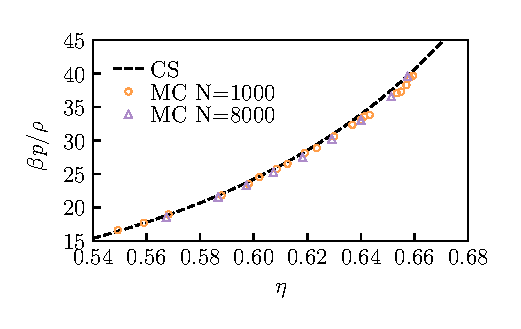
\includegraphics[width=0.9\linewidth,outer]{swap-cs-santos}
  \caption[Accuracy of Carnahan-Starling equation at high densities]{
    Accuracy of empirical Carnahan-Starling (CS) equation of state \eqref{eq:cs-mixtures} in the supercooled regime from comparison with novel Monte-Carlo (MC) simulations for a system with 23\% polydispersity.
    The size distribution of this system is described by \eqref{eq:berthier-size-measure}.
    The range of jamming volume fractions $\eta_J$ from non-equilibrium compression protocols with this system are indicated by the blue region.
    Simulation data and jamming densities reproduced from Ref.\ \cite{BerthierPRL2016}.
  }
  \label{fig:swap-eos}
\end{SCfigure}

Finally, we introduce the central approximation of chapters \ref{chapter:morphometric-framework}, \ref{chapter:morphometric-applications} and \ref{chapter:resummation} as a limit case of FMT.
The chemical potential of a new sphere $s$ can be determined as the free energy of a mixture where the limit where the new species is infinitely dilute, as in
\begin{equation}\label{eq:fmt-morphometric}
  \begin{split}
    \mu_s
    &=
    \lim_{\rho_s \to 0} \frac{\partial f^\mathrm{ex}}{\partial \rho_s}
    =
    \lim_{\rho_s \to 0}
    \sum_\alpha
    \frac{\partial n_\alpha}{\partial \rho_s}
    \frac{\partial f^\mathrm{ex}}{\partial n_\alpha},
    \\ &=
    \frac{\partial f^\mathrm{ex}}{\partial \xi_3} \frac{4 \pi R_s^3}{3}
    + \frac{\partial f^\mathrm{ex}}{\partial \xi_2} 4 \pi R_s^2
    + \frac{\partial f^\mathrm{ex}}{\partial \xi_1} R_s
    + \frac{\partial f^\mathrm{ex}}{\partial \xi_0}
  \end{split}
\end{equation}
using the explicit derivatives \eqref{eq:fmt-n-derivatives} in the second line.
Noting that the partial derivatives of $f^\mathrm{ex}$ are constants of the bulk liquid and the other contributions are normalisations of the intrinsic volumes (cf.\ Table \ref{table:geometric-quantities}), the central conjecture of the morphometric approach is that this generalises to arbitrary shapes; that is, the chemical potential can be written \cite{KonigPRL2004,RothPRL2006}
\begin{equation}\label{eq:fmt-morphometric-2}
  \mu_s = p V_s + a_2 A_s + a_1 R_s + a_0
\end{equation}
with thermodynamic coefficients $\{p, a_2, a_1, a_0\}$ independent of the geometry.
We leave detailed discussion of this approximation until chapter \ref{chapter:morphometric-framework}, but for reference we will give the explicit coefficients for the already introduced FMT functionals below.

The thermodynamic coefficients in \eqref{eq:fmt-morphometric-2} can be determined for an FMT functional using the special case of spherical solutes \eqref{eq:fmt-morphometric}.
For the Rosenfeld functional \eqref{eq:rosenfeld-functional} we obtain the thermodynamic coefficients for the single-component hard sphere liquid
\begin{subequations}\label{eq:rosenfeld-coefficients}
  \begin{align}
    \beta a_0^\mathrm{RF}
    &=
    -\ln{(1- \eta)},
    \\
    \beta a_1^\mathrm{RF}
    &=
    \frac{6\eta}{\sigma (1 - \eta)},
    \\
    \beta a_2^\mathrm{RF}
    &=
    \frac{6\eta + 3\eta^2}{2\pi \sigma^2 (1 - \eta)^2},
    \\
    \frac{\beta p^\mathrm{RF}}{\rho}
    &=
    \frac{1 + \eta + \eta^2}{(1 - \eta)^3}.
    \label{eq:py-pressure}
 \end{align}
\end{subequations}
and for the CS functional \eqref{eq:santos-fmt} with \eqref{eq:cs-fmt} we find
\begin{subequations}\label{eq:wbii-coefficients}
  \begin{align}
    \beta a_0^\mathrm{WBII}
    &=
    - \ln{(1 - \eta)},
    \\
    \beta a_1^\mathrm{WBII}
    &=
    \frac{2}{\sigma} \left(
    \frac{5\eta + \eta^2}{1 - \eta}
    + 2 \ln{(1 - \eta)}
    \right),
    \\
    \beta a_2^\mathrm{WBII}
    &=
    \frac{1}{\pi \sigma^2} \left(
    \frac{\eta (2 + 3\eta - 2\eta^2)}{(1 - \eta)^2}
    - \ln{(1 - \eta)}
    \right),
    \\
    \frac{\beta p^\mathrm{WBII}}{\rho}
    &=
    \frac{1 + \eta + \eta^2 - \eta^3}{(1-\eta)^3},
 \end{align}
\end{subequations}
We label these as the White Bear II (WBII) coefficients because they were first derived from the WBII free energy functional%
\marginfootnote{These are not exactly as stated in Ref.\ \cite{Hansen-GoosJPCM2006} because we use a different definition of surface.
  The conversions between the different surfaces are stated in chapter \ref{chapter:morphometric-framework}: see the discussions around \eqref{eq:exclusion-transform}.}
\cite{Hansen-GoosJCP2006, Hansen-GoosJPCM2006} which is similar in form and construction to the CS functional described, although it is (marginally) less self-consistent.

%% \subsection{Superposition and convolution approximations}

%% \todo{Finish this section}
%% In the Kirkwood superposition approximation \cite{KirkwoodJCP1935} many-body correlations are expressed as pairwise products of the two-body correlation function, i.e.
%% \begin{equation}
%%   g^{(n)}(\vec{r}^n) =
%%   \prod_{i < j} g^{(2)}(\vec{r}_i, \vec{r}_j),
%% \end{equation}
%% which correctly satisfies the hard-core condition, but violates the sum rule
%% \begin{equation}
%%   \begin{aligned}
%%     \rho^{(n)}(\vec{r}^n) &=
%%     \frac{1}{\Xi} \sum_{N=n}^\infty \frac{z^N}{(N-n)!} \int e^{-\beta U_N} \, d\vec{r}^{(N-n)} \\
%%     &=
%%     \int d\vec{r}_n \left(
%%     \frac{1}{\Xi} \sum_{N=n}^\infty \frac{z^N}{(N+1 - (n+1))!} \int e^{-\beta U_N} \, d\vec{r}^{(N-(n+1))}
%%     \right) \\
%%     &=
%%     \int d\vec{r}_n \left(
%%     \frac{1}{\Xi} \sum_{N=n}^\infty \frac{z^N}{(N - (n+1))!} \int e^{-\beta U_N} \, d\vec{r}^{(N-(n+1))}
%%     \right) \\
%%     &=
%%     \frac{1}{N-n}
%%     \int \rho^{(n+1)}(\{\vec{r}^n, \vec{r}_{n+1}\}) d\vec{r}_{n+1},
%%   \end{aligned}
%% \end{equation}\todo{This is wrong.}
%% and the related convolution approximation \cite{JacksonRMP1962,IchimaruPRA1970,BarratMP1988}%
%% \todo{Check this expression is correct - it almost certainly is not.}
%% \begin{equation}
%%   S^{(n)}(\vec{k}^n) =
%%   (1 + \widetilde{c}^{(n)}(\vec{k}^n))
%%   \prod_{i < j} S^{(2)}(\vec{k}_i, \vec{k}_j)
%% \end{equation}
%% satisfies the sum rule but fails to satisfy the hard-core condition.

%% In equilibrium
%% \begin{equation}
%%   c^{(n)}(\vec{r}^n) =
%%   \left.
%%   \frac{\delta^n \beta F_{ex}}{\delta \rho(\vec{r}_1)\delta \rho(\vec{r}_2) \cdots \delta \rho(\vec{r}_n)}
%%   \right|_{\rho(\vec{r})=\rho}
%% \end{equation}


\ifdefined\includebibliography
  \newgeometry{margin=1in}
  \printbibliography
\fi

\end{document}
